\chapter{Corruption and Procurement Markets}

\section{Prelude}

In this chapter we map public procurement markets as bipartite networks of issuers (alternatively buyers, public institutions) and winners (suppliers, firms) of contracts. Using corruption risk indicators, we study the relationship between corruption risk and micro-, meso-, and macro-level structure of markets. We find that corruption risk is related to various structural properties of the market captured by its network structure, and that important heterogeneities exist among EU countries. We present findings using a dataset of over four million contracts awarded across the European Union between 2008 and 2016\footnote{This chapter partially draws on work that is under review at a journal at the time of submission of the thesis~\cite{fazekas2017corruption}. A preprint is available at ~\url{http://www.govtransparency.eu/wp-content/uploads/2017/09/Fazekas_Wachs_Skuhrovec_CorruptionNetwork_Structure_in_CZ_HU_2017.pdf}.}.

Bipartite networks have been used to study a wide variety of phenomena involving two distinct sets of actors, for example buyers and sellers in markets~\cite{hernandez2018trust}, flowers and their pollinators~\cite{jordano2003invariant}, and cities and industries~\cite{bustos2012dynamics}. As public procurement markets consist of two kinds interacting of actors (issuers and winners), they fit into this paradigm. We create networks of buyers and suppliers at the national level and describe their structure using the tools of network science.

As in the case of unipartite networks, empirical bipartite networks often exhibit certain regularities that distinguish them from random networks. For example the nodes in such networks tend to have heterogeneous degree distributions, meaning that certain nodes sometimes referred to as hubs have orders of magnitude more connections than other nodes. We show that procurement markets are no exception to this observed pattern, having heterogeneous degree distributions among both winners and issuers.

Some of the most interesting empirical regularities observed in real-world networks extend beyond the node level, describing structures at so-called mesoscopic scales. One example of a structure commonly found in empirical networks is the so called core-periphery structure. By filtering a network for its most important connections, referred to as the core of the network, using the network topology we can simultaneously highlight key actors and measure the centralization of a network~\cite{dorogovtsev2006k,csermely2013structure}. Core-finding methods have been used to analyze networks of trade~\cite{mahutga2006persistence}, success in creative industries~\cite{cattani2008core}, and political organization~\cite{barbera2015critical}. We apply a method to our data that considers both the weight of connections between issuers and winners, and the bipartite nature of our networks. Besides distinguishing important actors in the market, the relative size of the core and the share of contracts between core members is a measure of the centralization of a market. Indeed we find that there is a significant variation in the share of contracts between core issuers and firms across the EU countries.

Another example of mesoscopic network structure that occurs frequently in empirical networks is \textit{modularity}. As we saw in the previous chapter, social networks are often modular~\cite{newman2006modularity} because of factors such as homophily or social segregation~\cite{kossinets2009origins}. Modularity in a network derived from market interactions merits its own interpretation. It may indicate the degree of specialization in a market - i.e. if firms tend focus on providing a narrower set of goods and services - or the effects of geography. Using a method adapted especially for bipartite networks, we partition procurement markets into communities and find that they have significant modularity. We then analyze the distribution of corruption risk across the different modules of a market. Corruption risk may be concentrated in a few specific sectors, or it may be spread rather evenly throughout the entire market.

Combined with the overall prevalence of corruption risk in a country, we are able to describe in much more detail the shape of corruption risk and its organization using these methods. While two countries may have the same overall level of corruption risk in their public contracting, its distribution can be different. In one case the corruption risk may be highly clustered in certain communities and more common in the periphery of the market. In another, corruption may be evenly spread around the market, with no specific hot-spots of corruption, and on average more common in its core. Such an perspective offers a powerful diagnostic tool to researchers of corruption. Certainly effective prescriptions to combat corruption would be different in these two cases.

To emphasize the dynamics of corruption risk, we also analyze how changes in government effect high corruption risk winners in the core of the network. We test the survival of winning firms across two years intervals, finding that in some countries winners are more stable across changes of government, while in others they are less likely to survive. More abstractly speaking, this analysis quantifies the political organization of corruption in the different EU countries.

We proceed by introducing the data, describing how it can be represented as a bipartite network, defining measures of the resulting networks, and comparing network structure with corruption risk indicators. We find significant differences between countries, beyond what can be explained by differences in the overall prevalence of corruption risk. We conclude with a discussion of these findings.

\section{Data}
Our data is collected from \textit{Tenders Electronic Daily}\footnote{\url{https://ted.europa.eu/}} 
(TED) - the official journal of public procurement contracts of the European Union. TED includes both calls for tenders and award announcements of contracts from all member states in the European Union. TED estimates the total value of tenders published in a year is worth approximately 420 billion Euro - a significant share of EU GDP (2.8\% in 2016). EU law requires, with some rare exceptions, that all public procurement contracts estimated in value above a certain threshold issued by member states be reported on the website. In 2016 these thresholds were $135,000$ Euro for service and supply contracts, and 5.2 million Euro for works contracts. Though a significant amount of procurement takes place below this threshold (and in most cases is recorded in national or regional level data portals), we use only TED data above the threshold in order to maximize cross-national comparability. One drawback to our use of TED is that corrupt actors have significant incentives to issue contracts just under the reporting threshold~\cite{szucs2017discretion}, leading to an underestimation of corruption risk in certain countries or markets. 

Our dataset consists of 4,098,711 contracts awarded between 2008 and 2016 from 26 member states of the EU\footnote{We exclude Luxembourg because it issues relatively very few contracts, and Croatia because it joined the EU only in 2013.}. We exclude contracts awarded by the European Institutions, for example the European Commission and European Parliament, as we are interested in a comparison between countries. As issuers and winners of public contracts are named by raw text string at the contract level, and not by unique identifiers (i.e. by EU VAT ID or other national tax ids), we first created an algorithm to identify and merge aliases referring to the same issuers and winners, country by country. In the computer science literature, such a task is known as deduplication or record-linkage. Deduplication in general is a difficult problem because comparing all pairs of $N$ potentially distinct entities will require in general on the order of $N^{2}$ comparison. Our method follows the overall approach outlined by Christen~\cite{christen2012data}, consisting of five steps:

\begin{itemize}
    \item Preprocessing: we process at the contract level each issuer and winner's name, street address, postal code, and country fields by lower-casing all characters and removing punctuation and superfluous white space. 
    \item Choosing a measure of similarity: we quantify the similarity of two entities using an active learning approach~\cite{sarawagi2002interactive} implemented in the \textit{Dedupe} Python programming library~\cite{gregg2015dedupe}. For each field in a record, the method defines several measures of similarity. For instance, the text names of two winners can be compared using a measure of string edit distance (counting for instance the number of insertions and deletions required to transform one string into another), the overlap of shared words, or the similarity of the first characters in each word. The algorithm selects a small sample of pairs of records and calculates a large number of similarity measures. It presents the user with those examples of pairs of records which it is most unsure about. The algorithm learns both which similarity measures are productive in the classification of pairs of records and how and in what proportion they should be combined to achieve the best accuracy. By labeling 100 such examples, the user can greatly increase the accuracy of the deduplication procedure. We ran this algorithm and manually classified 100 examples for both winners and issuers for each country in our dataset.
    \item Choosing records to compare: As mentioned, there are many possible records to compare. Comparing all pairs of 1,000 records for example would require making roughly 500,000 comparisons. France alone has 364,125 unique winner names. Moreover, since the method of comparing records learned in the previous step requires the calculation of multiple measures of similarity, it is important to reduce the space of searches in a clever way. This is accomplished via a technique called blocking: the records are split into groups based on simple features such as sharing the same first three characters in their name (i.e. Microsoft and Microsystems would be placed in the same block) or sharing the same first character in the first two tokens of their names (i.e. Air France and Air Finland would be placed in the same block). Blocking is not a strict partition: records can be placed in multiple blocks. Using the same sample of manually labeled candidate matches, the computer program learns which blocks are most effective for maximizing the trade-off between accuracy and the number of comparisons that need to be calculated.
    \item Grouping similar records: Once the similarity of records for all pairs of issuers or winners in all blocks have been calculated, we use a hierarchical clustering method to determine which records should be identified as duplicates.
    \item Selecting a threshold in the clustering:  Again, relying on the manually checked sample of records we select a threshold that weighs false positives (i.e. two records which do not refer to the same entity in reality, but are merged) and false negatives (i.e. two records which refer to the same entity in reality but are not merged) equally. The overall accuracy of our approach, while varying for issuers and winners and country by country, exceeds 90\% on the sample of difficult to classify cases identified by the software. The number of unique winners in France, for example, decreases from 364,125  to 200,584 after the procedure.
\end{itemize}

Equipped with this deduplicated set of issuers and winners, we can, with significantly greater confidence, represent the interactions between actors as a network. We are also interested, of course, in quantify corruption risk at the contract level, as we did in the previous chapter. Unfortunately, data inconsistency across both time and countries in the TED data limit us in this regard. After an evaluation of the various potential corruption risk indicators, their stability over time within countries, and the rate at which data was missing, we concluded that a single indicator - single bidding - was the most appropriate measure of corruption risk. We have already presented the correlations between this measure, aggregated over time, and other perception-based measures of corruption risk in Chapter 2, finding a national level correlation between the rate of single bidding and measures such as Transparency International's Corruption Perceptions Index and the World Bank's Control of Corruption measure of between .6 and .7.


\section{Markets as Bipartite Networks}
Given a collection of contracts awarded by issuers to winners from a given country in a year, we construct a network as follows. The nodes consist of issuers and winners of public contracts. An issuer and winner are connected by an edge if they are in a contracting relationship that year. The edge has a weight, initialized at 1, that increases in the count of contracts entered between the issuer and winner. We note that this network is ~\textit{bipartite}, that is consisting of two nodes sets within which there are no edges, i.e. there are no connections between two winners or two issuers\footnote{In the rare case that a public institution also wins contracts as a supplier entity, we split the institution into two nodes: one capturing its role as an issuer, the other as a winner of contracts.}. Each edge also encodes the single bidding rate of contracts between the given issuer and winner. We visualize a toy example of such a bipartite network in Figure~\ref{fig:toynetwork}.

\begin{figure*}[t]
\centering
  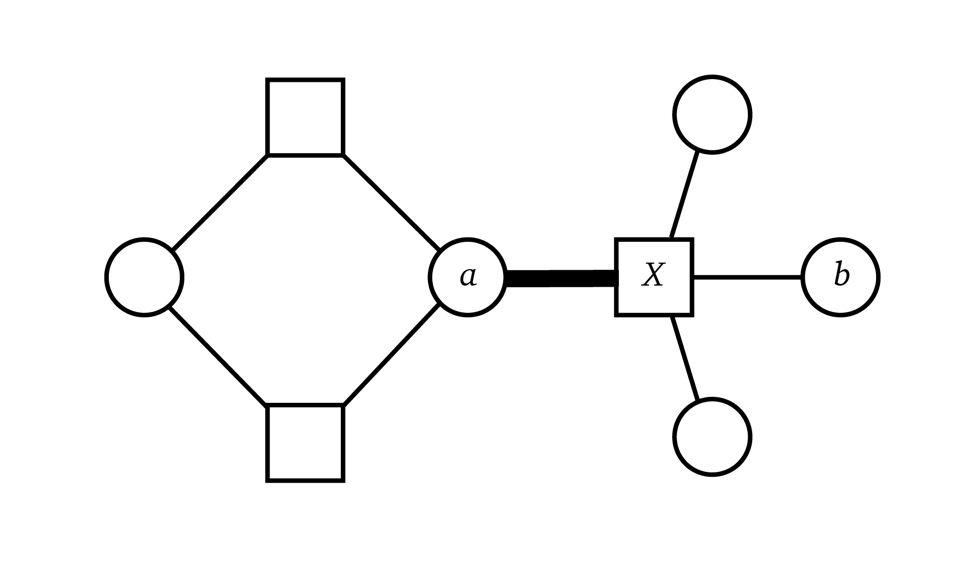
\includegraphics[width=\textwidth]{images/ted_networks/toy_network.png}
  \caption[Toy bipartite network.]{A toy example of a public procurement market represented as a bipartite network. Squares represent issuers and circles represent winners of public procurement contracts. For instance, winners a and b are connected by edges with issuer X. The edge between a and X is thicker than the edge between X and b, indicating that a has won more contracts from X than b. Adapted from~\cite{fazekas2017corruption}.}
  \label{fig:toynetwork}
\end{figure*}

We proceed by calculating a few summary statistics about these networks, seeing if they conform to some of the regularities observed in other empirical networks which distinguish them from random networks.  We calculate the density of each network by dividing the number of edges present, over the number of edges in the complete bipartite graph with the same number of issuers and winners. We also calculate the averages and standard deviations of degrees of both nodesets. Finally, we calculate the Robins-Alexander clustering~\cite{robins2004small} of each network, a measure of local correlations in connectivity for bipartite networks, analogous to measures of triadic closure in monopartite networks such as social networks. 

Robins-Alexander clustering counts the number of four-cycles ($C_{4}$) in a network, defined as a path of edges between 4 nodes, starting and ending at the same node and visiting each node once. In the toy network visualized in Figure~\ref{fig:toynetwork}, the path starting and ending at a and visiting the nodes in the left part of the network is a four-cycle. The count of four-cycles is divided by the count of paths of length three, representing the number of potential four-cycles. This quotient is multiplied by 4 to account for the fact that each four cycle contains four paths of length 3. This measure is a direct generalization of the concept of the global clustering coefficient for monopartite networks~\cite{wasserman1994social,watts1998collective}, which in social networks measures the likelihood that if an individual has two friends, those two individuals are also friends with each other. As there are no triangles in bipartite networks, Robins-Alexander clustering is a natural extension of the concept from triangles to squares. 


We present some summary statistics of the networks of each country averaged over the period 2008-2016 in Table~\ref{tab:network_summary}. We first note that the number of contracts awarded and nodes participating in the market varies significantly from country to country. Despite this heterogeneity, in other regards all procurement markets seem to share properties typical of other empirical networks. The markets are sparse, with the number of observed connections well below the number of possible connections, as indicated by the low density. The networks have significant Robins-Alexander clustering, suggesting interdependence of nodes close to one another in the network. For both winners and issuers, the variance of their degrees exceeds the average of their degrees, a signal that the degree distribution for both node sets is heterogeneous.

\begin{landscape}
\begin{table*}[t]
\begin{tabular}{lrrrrrrrrr}
\toprule
Country &  \# Contracts &  \# Winners &  \# Issuers &  Density &  R-A Clust. &  $\mu$(Deg_{W}) &  \sigma(Deg_{W}) &  \mu(Deg_{I}) &  \sigma(Deg_{I}) \\
\midrule
AT      &        3314 &      1882 &       395 &   0.0033 &    0.03 &             1.8 &             2.3 &             8.4 &            22.7 \\
BE      &        6674 &      3046 &      1039 &   0.0014 &    0.02 &             2.2 &             4.4 &             6.4 &            15.2 \\
BG      &        8653 &      2150 &       484 &   0.0048 &    0.27 &             4.0 &            14.6 &            17.9 &            56.3 \\
CY      &         916 &       403 &        64 &   0.0179 &    0.14 &             2.3 &             3.7 &            14.3 &            48.7 \\
CZ      &        8030 &      2933 &       986 &   0.0017 &    0.04 &             2.7 &             7.4 &             8.1 &            32.7 \\
DE      &       32339 &     15395 &      4049 &   0.0004 &    0.03 &             2.1 &             5.2 &             7.9 &            23.5 \\
DK      &        4858 &      2099 &       539 &   0.0028 &    0.04 &             2.3 &             4.1 &             8.9 &            26.5 \\
EE      &        1913 &       967 &       170 &   0.0083 &    0.08 &             2.0 &             2.6 &            11.0 &            28.9 \\
ES      &       20035 &      7496 &      1765 &   0.0011 &    0.13 &             2.7 &             6.8 &            11.3 &            31.8 \\
FI      &        6248 &      2750 &       578 &   0.0029 &    0.05 &             2.3 &            12.2 &            10.8 &            27.4 \\
FR      &      120946 &     42562 &      6294 &   0.0003 &    0.08 &             2.8 &            11.5 &            19.3 &            51.4 \\
GR      &        4246 &      2348 &       437 &   0.0031 &    0.12 &             1.8 &             2.2 &             9.7 &            44.0 \\
HU      &        5700 &      2016 &       610 &   0.0026 &    0.08 &             2.8 &             5.9 &             9.4 &            27.4 \\
IE      &        2713 &      1587 &       208 &   0.0056 &    0.03 &             1.7 &             2.3 &            13.1 &            51.3 \\
IT      &       18249 &      7749 &      2434 &   0.0006 &    0.07 &             2.4 &             7.2 &             7.5 &            29.0 \\
LT      &        9007 &      1368 &       272 &   0.0084 &    0.32 &             6.5 &            40.2 &            32.5 &           178.2 \\
LV      &        9451 &      2148 &       262 &   0.0057 &    0.15 &             4.3 &            14.8 &            36.1 &           119.4 \\
NL      &        6691 &      3579 &      1136 &   0.0013 &    0.02 &             1.8 &             2.6 &             6.0 &            14.7 \\
NO      &        3479 &      1899 &       497 &   0.0031 &    0.04 &             1.8 &             2.7 &             7.0 &            12.6 \\
PL      &      108886 &     19079 &      3649 &   0.0006 &    0.23 &             5.7 &            64.7 &            29.7 &            96.9 \\
PT      &        2255 &      1052 &       334 &   0.0041 &    0.08 &             2.1 &             3.1 &             6.7 &            30.4 \\
RO      &       19807 &      3503 &       939 &   0.0025 &    0.32 &             6.0 &            44.5 &            21.1 &            72.5 \\
SE      &        9441 &      4721 &       724 &   0.0022 &    0.06 &             2.0 &             3.7 &            13.1 &            33.3 \\
SI      &        6623 &      1268 &       448 &   0.0067 &    0.27 &             5.2 &            18.7 &            14.8 &            33.3 \\
SK      &        2654 &      1068 &       344 &   0.0043 &    0.09 &             2.4 &             5.1 &             8.1 &            32.5 \\
UK      &       32275 &     15577 &      2230 &   0.0006 &    0.04 &             2.1 &             3.7 &            14.6 &            50.0 \\
\bottomrule
\end{tabular}
\caption[Procurement Market Network Summary Statistics]{Summary statistics of procurement market networks, averaged over 2008-2016. R-A Clust. refers to Robins-Alexander clustering, a measure of the local correlation of connectivity in bipartite networks, analogous to triadic closure in monopartite networks. The final four columns present the averages and standard deviations of winner and issuer degree (weighted by contract count), respectively.}
\label{tab:network_summary}
\end{table*}
\end{landscape}

In order to investigate the heterogeneity of the degree distributions further, we plot distribution of the number of contracts awarded and won by each issuer and winner, respectively, pooled across the entire EU in Figure~\ref{fig:eu_dists}. Using the method described by Clauset et al. ~\cite{clauset2009power,alstott2014powerlaw} we estimate the best fit alpha of a power-law distribution for both distributions, estimating an alpha of 2.27 for winners and 2.16 for issuers. In both cases a statistical test between the goodness of fit of a powerlaw distribution compared with a lognormal distribution is inconclusive: neither one is significantly better. What is clear, however, is that both node sets have extremely heterogeneous distributions, with most winners and issuers participating in very few contracts, while a few winners and issuers participate in over a thousand contracts. This sort of heterogeneity is a typical characteristic of empirical networks and has significant implications for their structure.

\begin{figure*}[!t]
\centering
  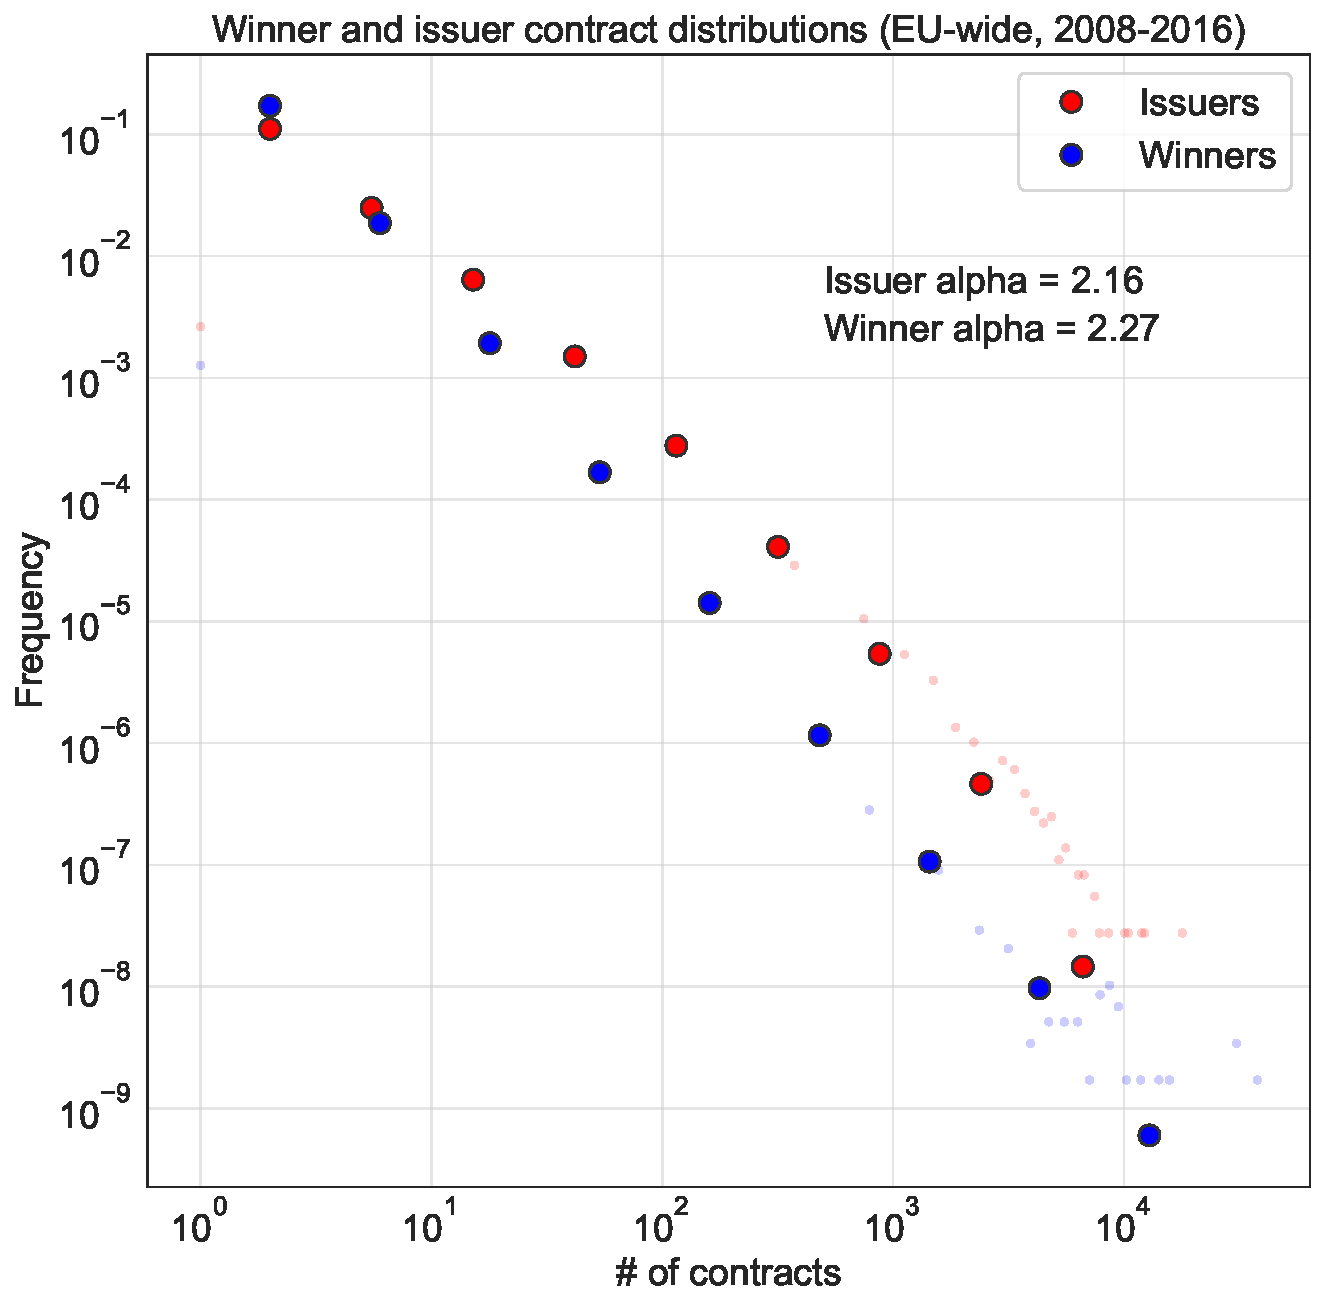
\includegraphics[width=\textwidth]{images/ted_networks/eu_df_global_dists.pdf}
  \caption[Contract distributions of issuers and winners, EU-wide.]{The distribution of the number of contracts awarded and won, for issuers and winners, respectively, of procurement contracts across the entire EU. The distributions are plotted on a log-log scale. We report the alpha parameter of a power-law degree distribution fitted to both distributions in the plot.}
  \label{fig:eu_dists}
\end{figure*}


We repeat this visualization and calculation at the country level in Figure~\ref{fig:national_dists}. We observe remarkable regularity in the distributions of issuers and winners across countries. In all countries, both distributions are highly heterogeneous - the number of contracts issued or won by nodes ranges across several orders of magnitude. 

\begin{figure*}[!t]
\centering
  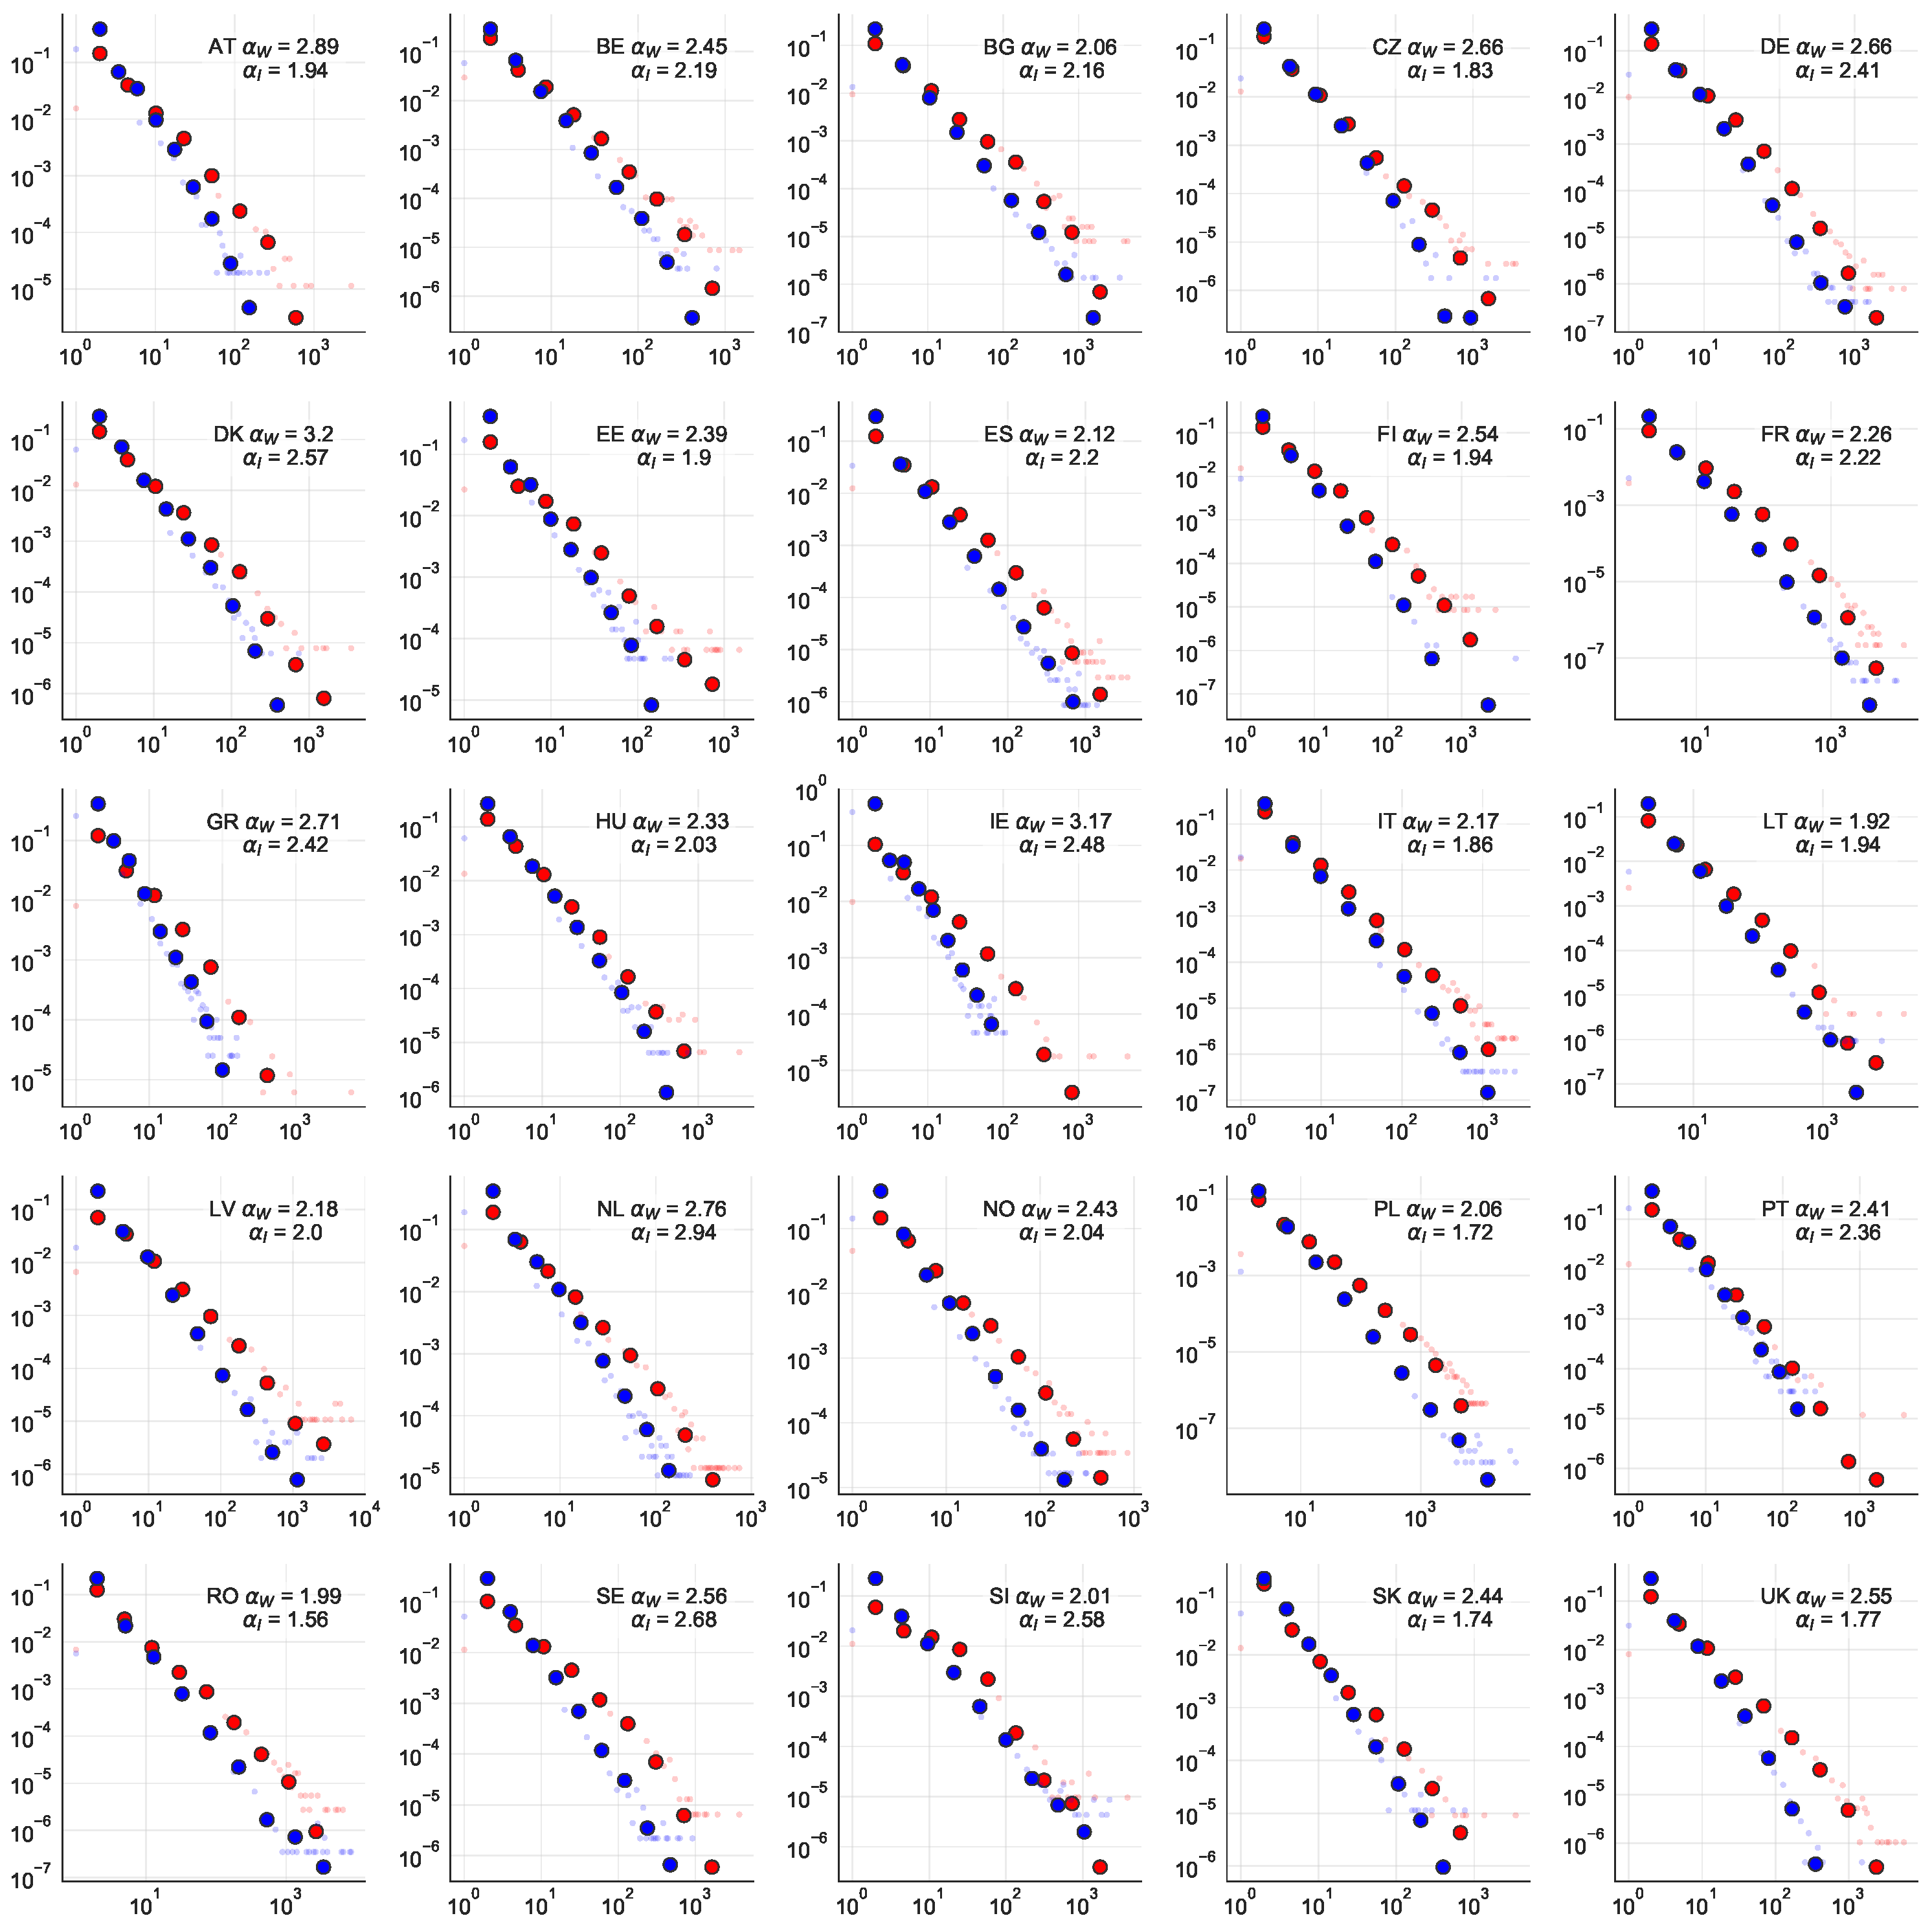
\includegraphics[width=\textwidth]{images/ted_networks/df_eu_national_dists.pdf}
  \caption[Contract distributions of issuers and winners, Country-level.]{The distribution of the number of contracts awarded and won, for issuers (in red) and winners (in blue), respectively, of procurement contracts in each country, aggregated from 2008 to 2016. The distributions are plotted on a log-log scale. We report the alpha parameter of a power-law degree distribution fitted to both distributions in the plot.}
  \label{fig:national_dists}
\end{figure*}

So far we have observed several regularities in the network structure of the EU national procurement market networks. These indicate in some sense why analyzing these markets as networks may be a fruitful endeavour: structure in these networks deviates significantly from what one would expect in networks with the same number of nodes and edges and uniform random probability. Such networks do not have significant clustering, nor do they have significant heterogeneity in their degree distributions. We now proceed with a study of these networks that is theoretically relevant to market structure and the distribution of corruption risk in them.


\subsection{The Core of Procurement Markets}
Given the size and complexity of these markets when modeled as networks, it is natural to ask if they can be filtered or simplified in a way that highlights the most central and significant actors and interactions. Networks often have such a center or \textit{core} which is essential to its functioning~\cite{csermely2013structure}. It is unclear if public procurement markets have such a core-periphery structure. Likely this depends on the organization of the market, for example if the procurement contracts are awarded in a centralized or decentralized manner in a country. Detecting the core of procurement markets and measuring their relative sizes offers us a way to highlight important issuers and winners, and more generally how centralized the market is. This itself would be a valuable measure as we can revisit a major debate in the corruption literature, which asks if that centralization in government is correlated with worse corruption outcomes, from a novel perspective.

Most comparative studies relating the centralization of government and corruption measured using perception-based indicators find a positive correlation~\cite{fisman2002decentralization,gurgur2005localization}: corruption is more prevalent in countries in which the responsibilities of government are concentrated in a few institutions. A theoretical model by Persson and Tabbellini proposes one possible mechanism, namely that centralization obscures political responsibility for corrupt outcomes~\cite{persson2002political}. In their model, politicians are reelected based on how well voters think they are doing their jobs. In a decentralized system responsibility is more closely tied to individuals, more directly linking good performance (abstaining from corruption) with rewards (reelection). In a centralized system it is harder for voters to observe which politicians are responsible for which outcomes. Yet Charron et al. find that within country variance of the EQI quality of governance indicator is not correlated with government centralization~\cite{charron2014regional}.

Going beyond the overall level of corruption risk in a country's procurement market, a decomposition of its participants into core and periphery allows us to test if corruption risk itself is centralized or decentralized in a given country. In the former case, the central government itself may be captured by corrupt interests~\cite{fazekas2017networks}, while in the latter case corruption may simply be an opportunistic action taken by less important actors. This is an important distinction which has been applied to the organization of corruption in organization~\cite{pinto2008corrupt} and among crooked police officers~\cite{lauchs2012resilience}.

There are many methods to extract key nodes in a network. A popular approach which considers not only a node's individual importance, but that of its neighbors as well, is known as core decomposition~\cite{batagelj2002generalized,csermely2013structure}. The general idea of core decomposition is to organize nodes of a given network into a hierarchical ranking according to their connectivity in an iterative way. Such methods have been used in biology~\cite{wuchty2005peeling}, economics~\cite{garas2012k}, and sociology~\cite{ugander2012structural}. We first introduce the concept of the and $k$-core of a monopartite, unweighted network. We then explain how to extend this concept to the particular case of weighted, bipartite networks, of which our mapping of public procurement markets are examples.


The core number of a node in a network is defined iteratively~\cite{batagelj2002generalized}. First we calculate the degree of each node. All nodes of degree 1 are assigned core number 1. We then remove all such nodes and recalculate the degree of all remaining nodes. In this new graph we assign core number 2 to any nodes with degree 1, and again remove them and repeat the procedure. The procedure ends when all nodes have been assigned a core number. The core number is a hierarchical ranking of the nodes which can be used to define the $k$-cores of a network. A $k$-core is the collection of nodes with core number at least $k$. Researchers are often interested in the maximal $k$-core of a network, defined as the highest value $k$ for which any nodes have core number $k$~\cite{alvarez2006large}.

One reason the $k$-core decomposition method is so popular is that there is an efficient algorithm to calculate the core number of all nodes in a network ($O(log(m))$ - where $m$ is the number of edges in a network~\cite{batagelj2003m}. For a broad survey of network core decomposition methods and applications we refer to the survey paper by Malliaros et al.~\cite{malliaros2019core}.

Applying a core decomposition method to public procurement markets require us to modify the definition of the original k-core algorithm in two ways: to consider the weights on the edges (encoding the frequency of the contracting relationship between an issuer and a winner) and the bipartite nature of the network. The latter factor is important because, as we saw in the previous section, the two node sets typically have distinct distributions. 

In order to incorporate edge weights into our approach to finding the core of procurement market networks, we follow a similar approach Garas et al. in their extension of the k-core method to weighted networks~\cite{garas2012k}. Rather than iteratively pruning the network based on the degree of the nodes, we do the same using node strength, defined as the sum of weights on edges adjacent to a node. As all of the edge weights in our networks are integers (as they are counts of contract awards), we are able to repeat the same pruning process describe above for unweighted networks: remove all nodes with strength equal to 1, recalculate the strengths, and repeat - assigning the corresponding weighted core-numbers to each node as they are pruned.

This leaves a question: at what weighted $k$-core number do we consider a node to be a member of the periphery? By introducing node strengths based on heterogeneous weights, it is very likely that the maximal weighted $k$-core will be very small~\cite{garas2012k}. We also want to apply the same method to networks of different sizes and compare the results, suggesting that we need to consider a cutoff that is a function of the distribution of the strength of the nodes, for example its average. A final concern is that the distribution of node strengths is different for issuers and winners in a given network.

We address these concerns by using separate weighted core number cutoffs for the two node sets, namely their averages. In other words, a winner (respectively issuer) is considered to be in the core if its weighted-core number is greater than the average weighted degree of all winners (issuers) in the network. Instead of applying the same cutoff across all countries (and across node sets), this cutoff adapts to the size of the network and the distributions of connectivity observed in them. We visualize the core of the Hungarian procurement market over time in Figure~\ref{fig:hu_core}, highlight connections with above average single bidding rates (relative to the whole market) in red. 

\begin{figure*}
\centering
  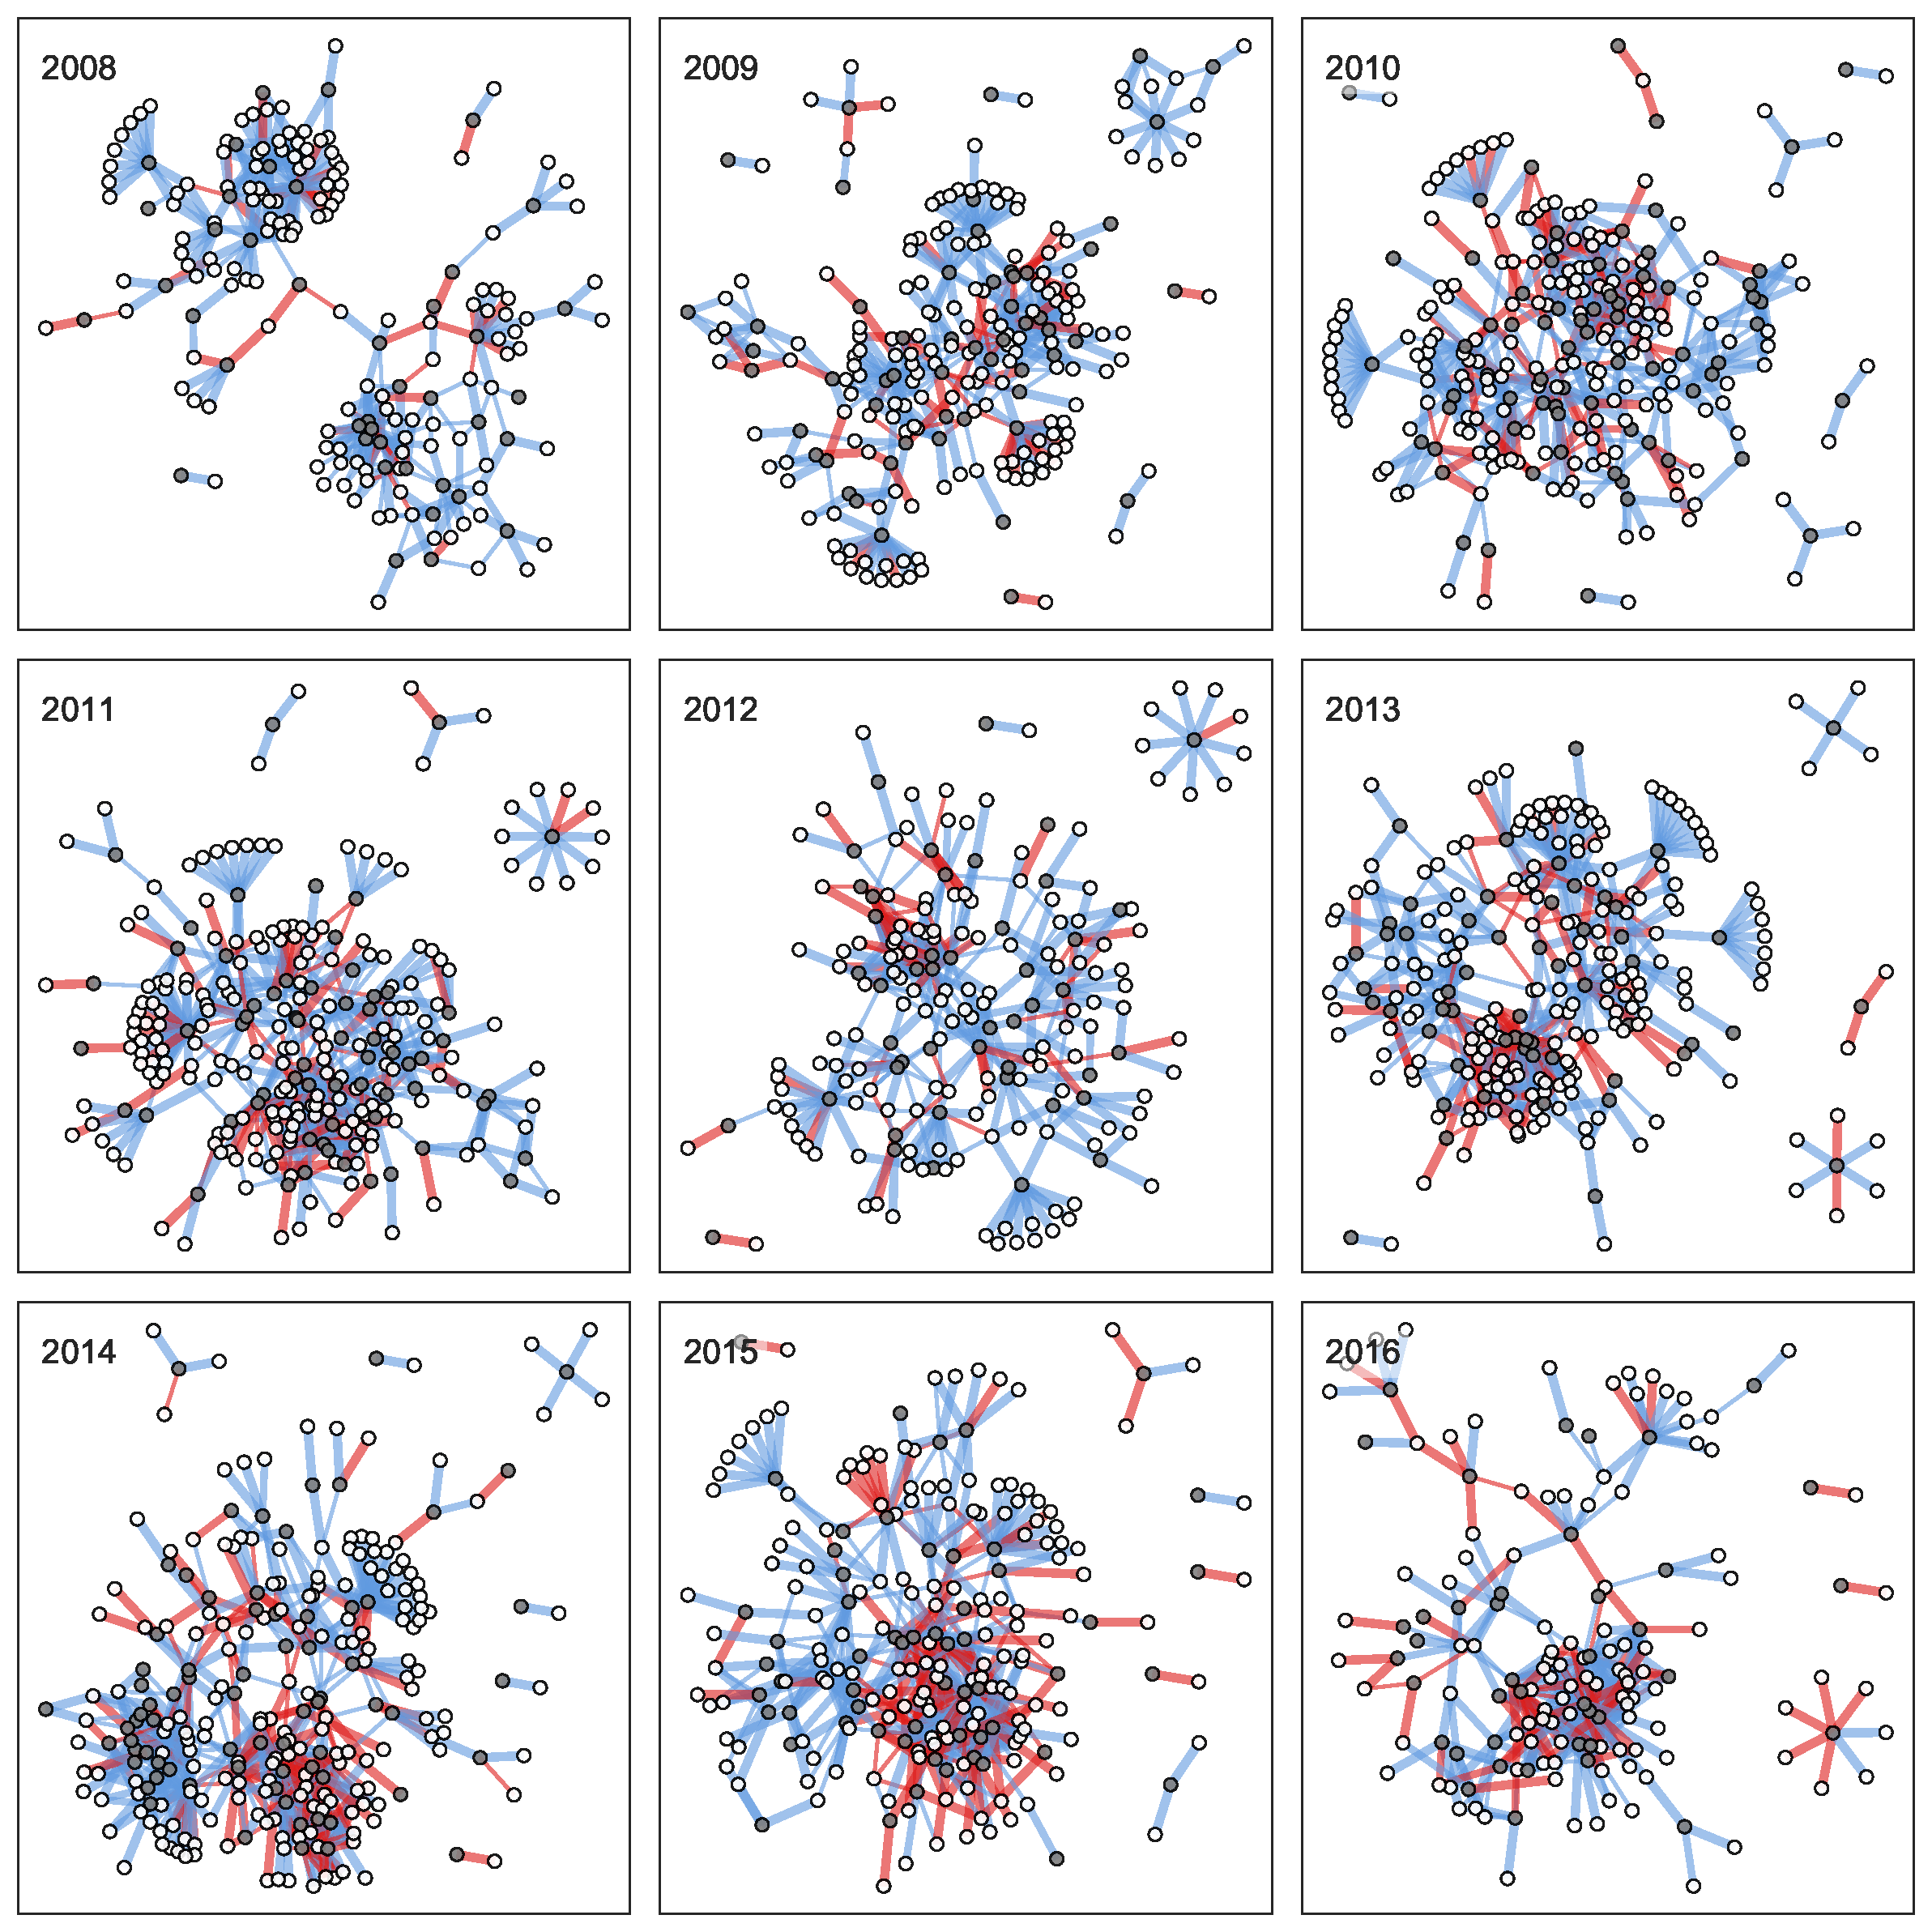
\includegraphics[width=\textwidth]{images/ted_networks/hu_core.pdf}
  \caption[Hungarian Market Cores]{The core of the Hungarian market from 2008 to 2016. Gray nodes denote issuers of contracts, while white nodes denote winners. Nodes are included in the core if they engage in many contracts with other highly active nodes, defined iteratively. Edges are colored red if the rate of single bidding on contracts between the issuer and winner exceeds the average single bidding rate observed in the whole market (including the periphery).}
  \label{fig:hu_core}
\end{figure*}

It is worth noting several things from this visualization. The first is that our adaptation of the general idea of $k$-cores to bipartite, weighted procurement market networks returns relatively dense networks. In other applications of $k$-core methods the density of connections among the core nodes is often highlighted to indicate that these nodes are distinguished in the network not only because they have many connections, but because they interact with other such nodes~\cite{malliaros2019core}. Second, the size of the core seems stable, indicating that the method itself is not overly sensitive to perturbations in the networks from year to year. On the other hand the mesoscopic structure of the network does seem to undergo interesting changes over time - compare the modularity of the core in 2008 with its concentration in 2015, echoing earlier research on the centralization of Hungarian procurement since 2010~\cite{fazekas2016corruption}. 

Finally, we note that the overall prevalence of high corruption risk edges in the core also seems to fluctuate. Recall that we color an edge red if the single bidding rate between the issuer and winner exceeds the total market average in that year. An increase in red edges in the core suggests that an increase in the frequency of single bidding in the core relative to the periphery. We first report summary statistics about the size of the cores in each country, averaged over the years in our data in Table~\ref{tab:core_stats}. 

\begin{table}
\begin{tabular}{lrrrrrr}
\toprule
Country &  Core \#Contracts &  Share &  \#Winners &  \#Issuers &  \#Edges &  \%Single bid.  \\
\midrule
AT      &              696 &                 0.21 &            111 &             25 &          168 &          0.14 \\
BE      &             1680 &                 0.25 &            188 &             92 &          382 &          0.14 \\
BG      &             3923 &                 0.44 &            162 &             61 &         1287 &          0.18 \\
CY      &              390 &                 0.42 &             32 &              3 &           41 &          0.39 \\
CZ      &             2764 &                 0.34 &            218 &             88 &          663 &          0.26 \\
DE      &             6973 &                 0.21 &            802 &            229 &         1827 &          0.16 \\
DK      &             1342 &                 0.27 &            147 &             45 &          323 &          0.11 \\
EE      &              441 &                 0.21 &             63 &             12 &          120 &          0.19 \\
ES      &             7182 &                 0.36 &            529 &            158 &         3206 &          0.18 \\
FI      &             1712 &                 0.27 &            167 &             50 &          661 &          0.15 \\
FR      &            39462 &                 0.32 &           2829 &            582 &        16345 &          0.14 \\
GR      &              715 &                 0.18 &            122 &             23 &          267 &          0.26 \\
HU      &             1949 &                 0.34 &            163 &             56 &          412 &          0.27 \\
IE      &              682 &                 0.24 &             91 &              9 &          111 &          0.02 \\
IT      &             6958 &                 0.38 &            462 &            156 &         1980 &          0.29 \\
LT      &             5414 &                 0.57 &             94 &             27 &          711 &          0.17 \\
LV      &             4664 &                 0.46 &            161 &             27 &          481 &          0.18 \\
NL      &             1137 &                 0.16 &            176 &             63 &          344 &          0.08 \\
NO      &              552 &                 0.15 &             87 &             28 &          233 &          0.06 \\
PL      &            66963 &                 0.61 &            896 &            455 &        14483 &          0.44 \\
PT      &              653 &                 0.26 &             67 &             20 &          116 &          0.22 \\
RO      &            12087 &                 0.59 &            165 &            106 &         2367 &          0.14 \\
SE      &             1761 &                 0.17 &            268 &             33 &          686 &          0.04 \\
SI      &             2632 &                 0.39 &             90 &             84 &          976 &          0.19 \\
SK      &              934 &                 0.34 &             68 &             28 &          144 &          0.37 \\
UK      &             8511 &                 0.25 &           1072 &            119 &         2058 &          0.08 \\
\bottomrule
\end{tabular}
\caption[Summary statistics of market cores.]{The core statistics of each national market, averaged over 2008-2016. Core share refers to the share of overall contracts awarded that are between core issuers and winners.}
\label{tab:core_stats}
\end{table}



In the rest of this section we probe these two aspects of the core of procurement markets: its size and the rate of single bidding of core contracts, relative to the whole market. The former allows us to quantify the centralization of procurement markets in a novel way, allowing us to revisit questions about the relationship between government centralization and corruption. The latter allows us to explore a potential heterogeneity in the prevalence of corruption across countries, namely if corruption risk is more common in the central actors of the procurement apparatus or in the periphery.

We plot the relationships between market centralization, measured as the share of all contracts which are between core issuers and winners, and both the single bidding rate, and the EQI QoG measurement in Figure~\ref{fig:centralization_vs_sb_eqi}. We find that the share of contracts in the core of the market predicts significantly higher corruption risk and lower quality of government. The correlation with the EQI quality of government measure is particularly high (.77). We interpret this as novel evidence in support of the theory that government centralization increases corruption. 

\begin{figure*}
\centering
  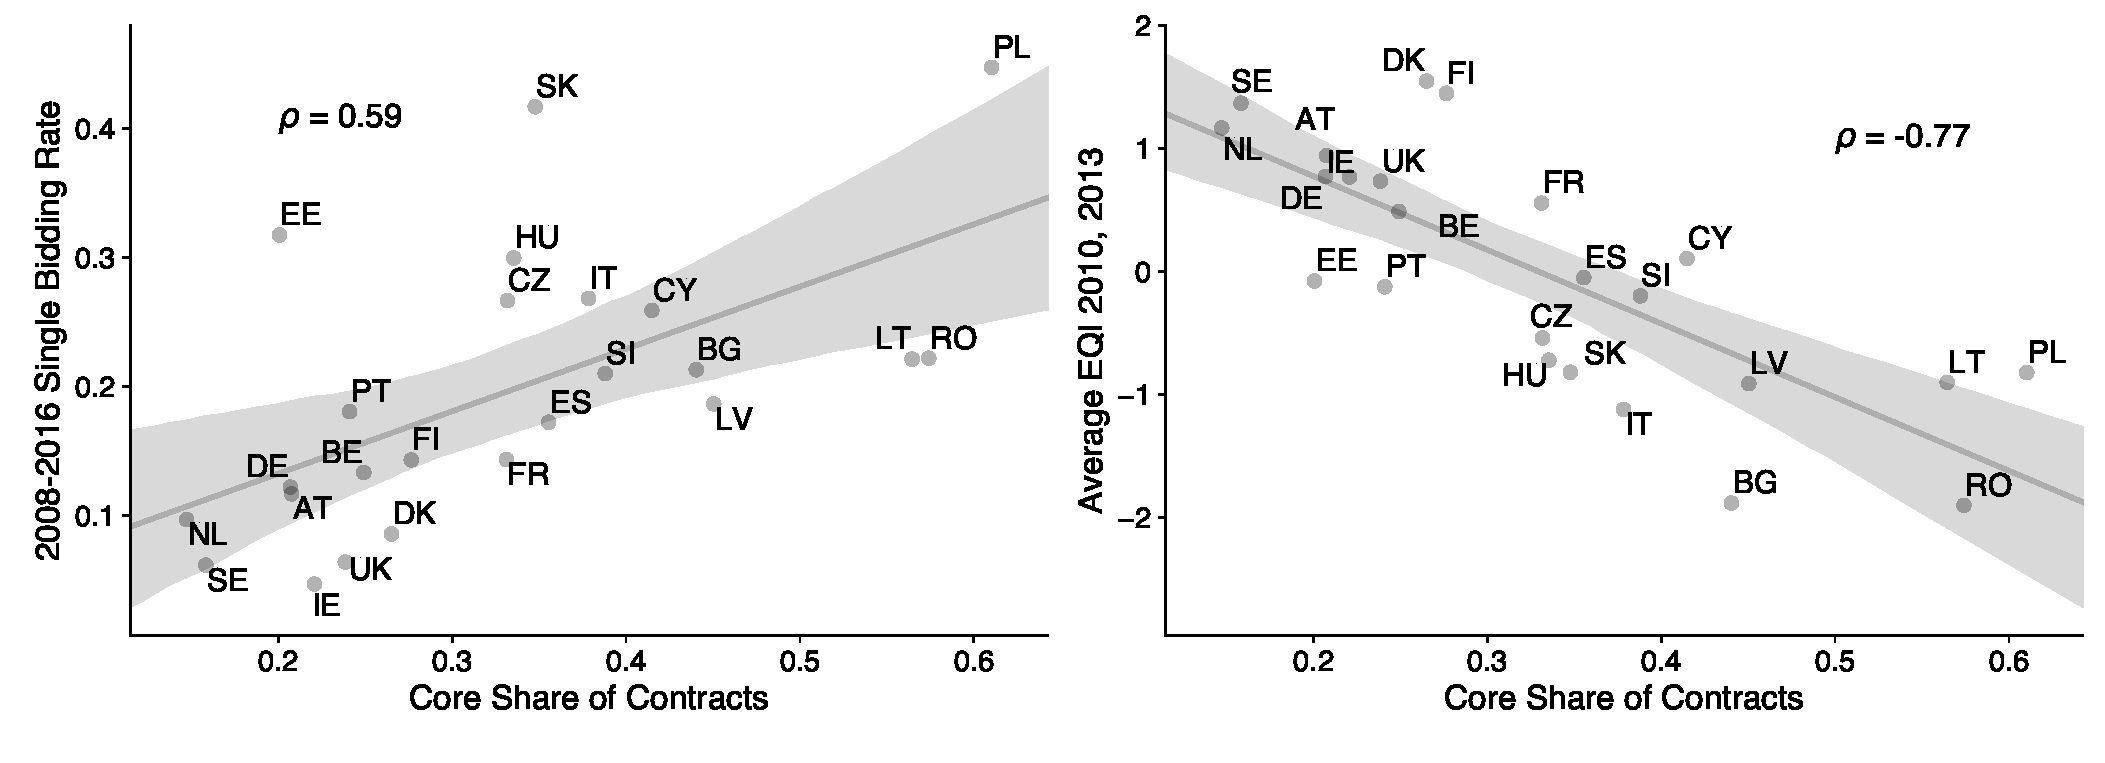
\includegraphics[width=\textwidth]{images/ted_networks/core_vs_sb_eqi.pdf}
  \caption[Market Centralization and Corruption]{Comparing the centralization of the procurement markets, measured as the share of all contracts which are between core issuers and winners, and measures of corruption risk at the national level. All measures are averaged over the years 2008-2016. We report Pearson correlations.}
  \label{fig:centralization_vs_sb_eqi}
\end{figure*}

In order to calculate the relative prevalence of single bidding in the core versus the periphery, we compare the observed relative prevalence of single bidding in the core to that of a null model with randomly shuffled single bidder labels. More specifically, we randomize single bidding at the contract level, then recalculate the rate of single bidding on contracts between core issuers and winners. In order to take into account market-specific effects (for instance markets for highly specialized services may have fewer firms, and so may have naturally higher rates of single bidding), we do not shuffle the single bidding labels freely across the entire market. We only permute labels within 2-digit CPV codes, which, as discussed in the previous chapters, are an EU-wide taxonomy of goods and services. Our measure of prevalence of single bidding in the core is the ratio of the observed single bidding in the core to the average of single bidding in the core in 1000 such randomized shuffles. In Figure~\ref{fig:core_sb} we highlight those countries with significant (at the 95\% confidence interval of the 1000 randomizations) over or under-representation of single bidding in their cores. 

\begin{figure*}
\centering
  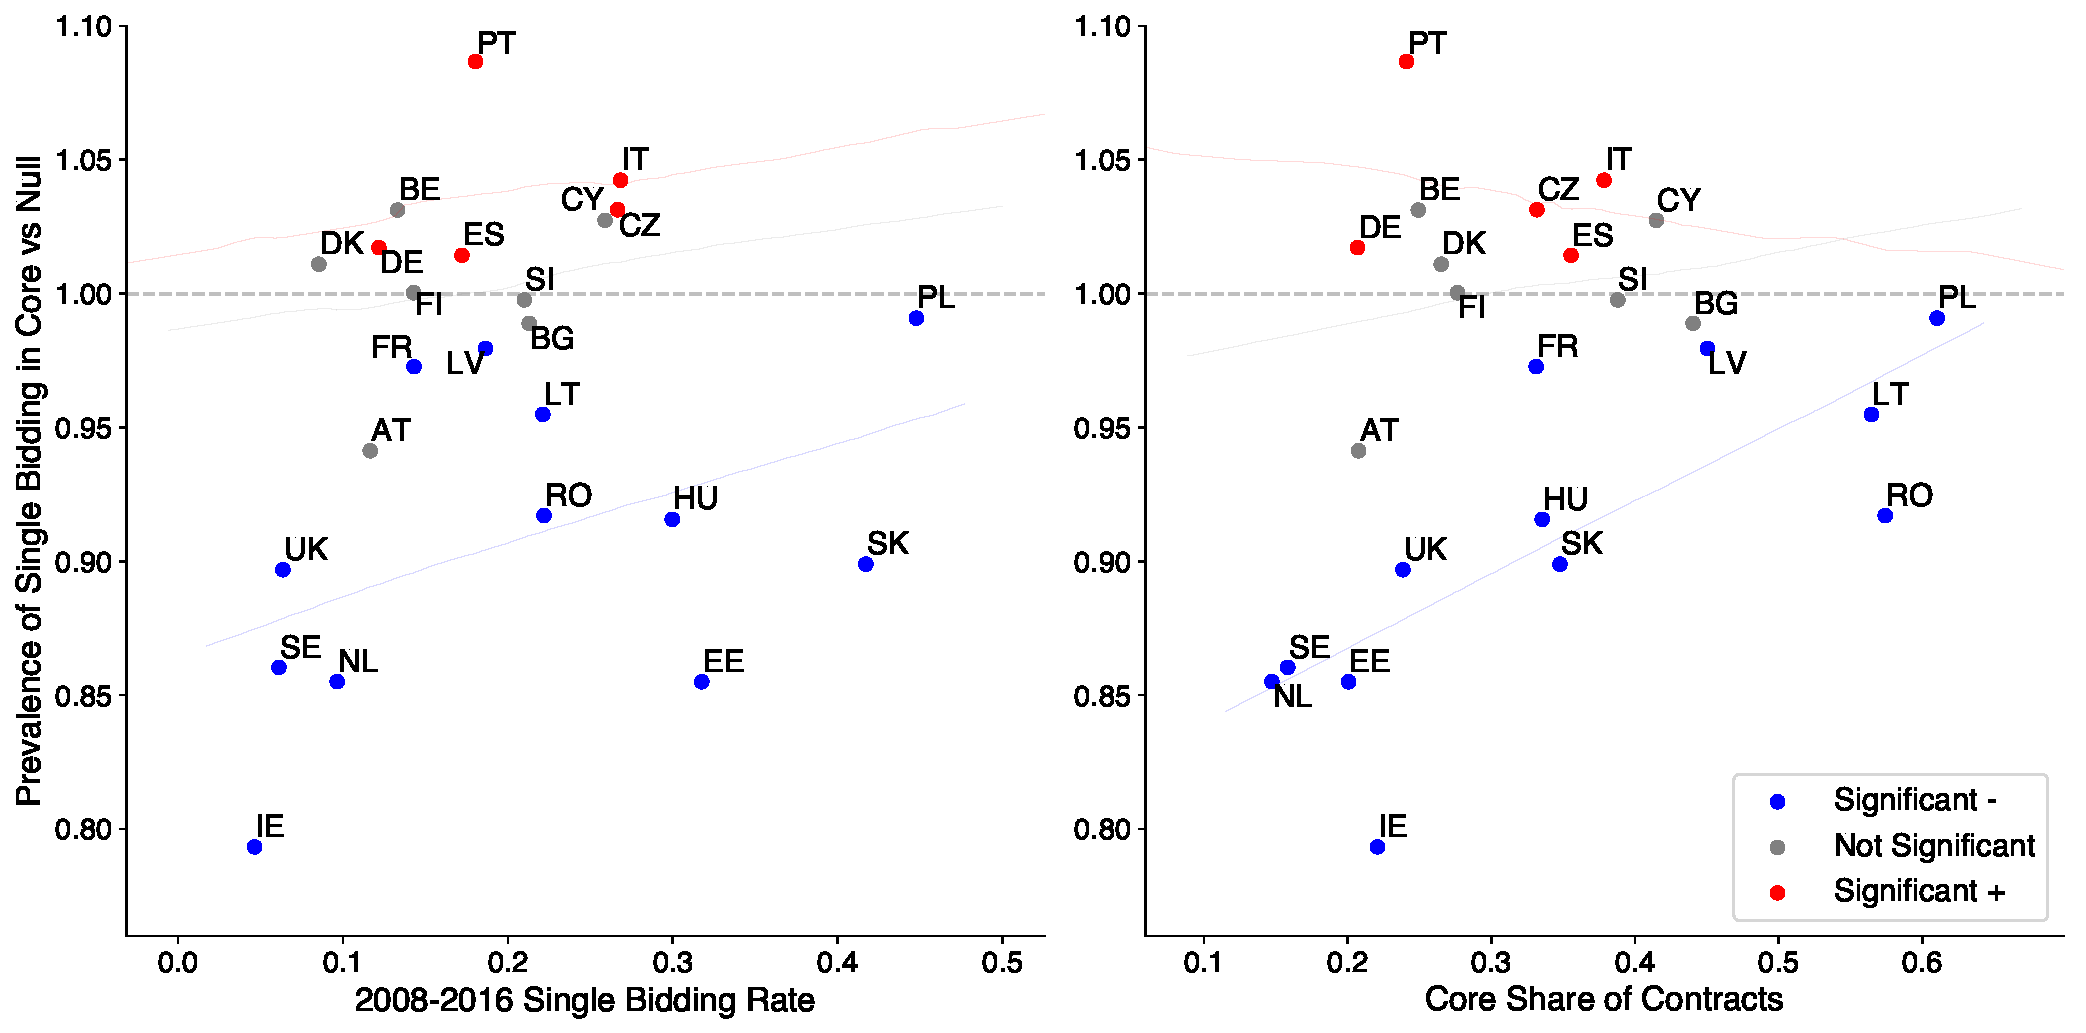
\includegraphics[width=\textwidth]{images/ted_networks/coresb_comparison.pdf}
  \caption[Prevalence of single bidding in cores.]{Comparing the relative prevalence of single bidding in the core of EU procurement markets with their overall single bidding rates and the relative core sizes, respectively. Blue points are countries in which single bidding is less common among core contracts than expected under a sector-preserving null model. Red points are countries in which the opposite is true: single bidding is significantly more common in core contracts.}
  \label{fig:core_sb}
\end{figure*}

We observe no clear linear relationship between a country's overall single bidding rate or its centralization and the tendency for single bidding to be more prevalent in the core or periphery. In Hungary and Slovakia, for instance, single bidding is more common in the periphery, while in Italy and Czechia, it is more common in the core of the market. In several countries including Bulgaria and Denmark, core rates of single bidding are not meaningfully different from the overall rate.

These findings contain important lessons for both policymakers and researchers of corruption. The concentration of corruption risk in the core or the periphery of a market suggests a very different organization of corruption in a society. Potential remedies likely depend on this distinction. For instance, if corruption is concentrated among core actors, as our findings suggest is the case in Italy and Czechia, checks on central government actors are likely lacking. When corruption is more common in the periphery, allocating more resources to policing corruption in local and regional governments or in geographically periphal areas may be more productive.

\subsection{The Clustering of Corruption Risk in Markets}
We now turn to a second question about the distribution of corruption risk in procurement markets: is corruption risk clustered? In other words: is corruption risk randomly distributed, or is it bunched up in certain parts of the network? We claim that answering this question is an important part of diagnosing the organization of corruption in a market and suggesting a remedy. If corruption risk is indeed clustered in specific parts of the market, targeted interventions in those areas will likely uncover useful information. In the case that corruption risk is randomly distributed, it would likely be more effective to reward whistleblowers.

How can we quantify the clustering of corruption risk in markets? We map this problem to a question of community detection, the process of grouping densely connected nodes in a network into modules~\cite{fortunato2010community}, as we did for social networks in Chapter 3. Again we must adapt the methods to our specific circumstances: corruption risk is a property of edges, and not of nodes. If we were to group nodes and calculate the heterogeneity of corruption risk across groups based on node-level data, it is not clear how one would handle corruption risk on edges between groups. Moreover, these edges are distinguished as bridges between groups of nodes, and would likely differ in some qualitative way from their intra-group counterparts. Ignoring them would bias any measure of the heterogeneity of corruption risk across groups.

Luckily there are several tried and tested methods to cluster the edges in a network into communities. Such ``link communities'' were originally used to cluster nodes into overlapping communities, i.e. nodes are members of all communities that their adjacent edges are assigned to. Specifically, we use the methods proposed by Evans and Lambiotte~\cite{evans2009line,evans2010line} and Ahn, Bagrow, and Lehmann~\cite{ahn2010link}, based on line graphs. The overall idea proceeds as follows: transform the graph in question into a new graph in which the edges of the original graph are now nodes, connected if they were adjacent in the original graph. Then by running a standard node-oriented community detection algorithm, such as the Louvain method described in the previous chapter~\cite{blondel2008fast}, to group the edges of the original graph. 

The line graph $L_{G}$ of a graph $G$ with vertices $V$ and edges $E$ is defined as a graph of nodes from $E$, connected if they have share a vertex from $V$. As edges adjacent to high degree nodes of the the graph $G$ will be significantly overrepresented in $L_{G}$, Evans and Lambiotte suggest to weigh the connections in $L(G)$ inversely proportional to the degree of their shared nodes in $G$. In other words, if $x$ and $y$ are edges in $G$ sharing a node $v$, hence nodes in $L(G)$, the edge connecting $x$ and $y$ is given a weight equal to $1/(deg(v)-1)$. This adjustment~\footnote{Evans and Lambiotte suggest a further adjustment in case the original graph $G$ is weighted which we leave for future work.} is motivated by the desire to maintain the consistency of the behavior of random walkers between $G$ and $L_{G}$. 

Given the network associated to a national procurement market, we transform the network into a line graph, and then apply the Louvain algorithm to cluster the edges. This assigns each contracting relationship, and indeed each contract within that relationship to a community. We list the average of the yearly modularities, a measure of the quality of the partition - that is the tendency of edges in the network to be within rather than between communities - defined in the previous chapter, calculated for each country in our dataset in Table~\ref{tab:edge_modularities}. In all cases we see very high levels of modularity, indicating that procurement markets typically have distinct submarkets. This is a reasonable finding considering that these markets include contracts for goods and services ranging from road construction to school milk to IT consultancy services, and likely have significant geographic influences.


\begin{table}
\begin{tabular}{lr}
\toprule
Country &  Edge Clustering Modularity \\
\midrule
SI      &           0.58 \\
LT      &           0.60 \\
BG      &           0.62 \\
RO      &           0.62 \\
PL      &           0.64 \\
ES      &           0.66 \\
FI      &           0.67 \\
FR      &           0.68 \\
NO      &           0.69 \\
SE      &           0.69 \\
HU      &           0.70 \\
DK      &           0.70 \\
CZ      &           0.70 \\
EE      &           0.70 \\
LV      &           0.71 \\
DE      &           0.72 \\
NL      &           0.72 \\
SK      &           0.73 \\
IT      &           0.73 \\
BE      &           0.73 \\
PT      &           0.73 \\
AT      &           0.74 \\
GR      &           0.75 \\
UK      &           0.75 \\
CY      &           0.76 \\
IE      &           0.79 \\
\bottomrule
\end{tabular}
\caption[Average National Procurement Market Edge-Clustered Modularity]{The average modularity of the edge-clustering of each national procurement market from 2008 to 2016. Large numbers indicate a more fragmented market topology.}
\label{tab:edge_modularities}
\end{table}


As an example, we plot the 2014 Hungarian market in Figure~\ref{fig:hu2014_edgecluster}. For simplicity of visualization we consider only those nodes in the giant component and involved in at least three contracts, and we color nodes by the most frequent edge community they are adjacent to. We color the edges red if the single bidding rate of contracts between those actors exceeds the market average that year. From this visualization we observe that single bidding seems to be clustered, particularly between actors in the top cluster. A manual inspection of the prominent issuers and winners in this group indicates that this is the health and pharmaceutical industry in Hungary. This is in significant contrast with the relatively few significant single-bidding edges seen in the top right cluster, containing several prominent food and drink providers. In contrast to the strong relationship between market centralization, measured by the share of contracts awarded in the core of the network, and overall market corruption risk, we find no significant relationship between market modularity and corruption risk.


\begin{figure*}
\centering
  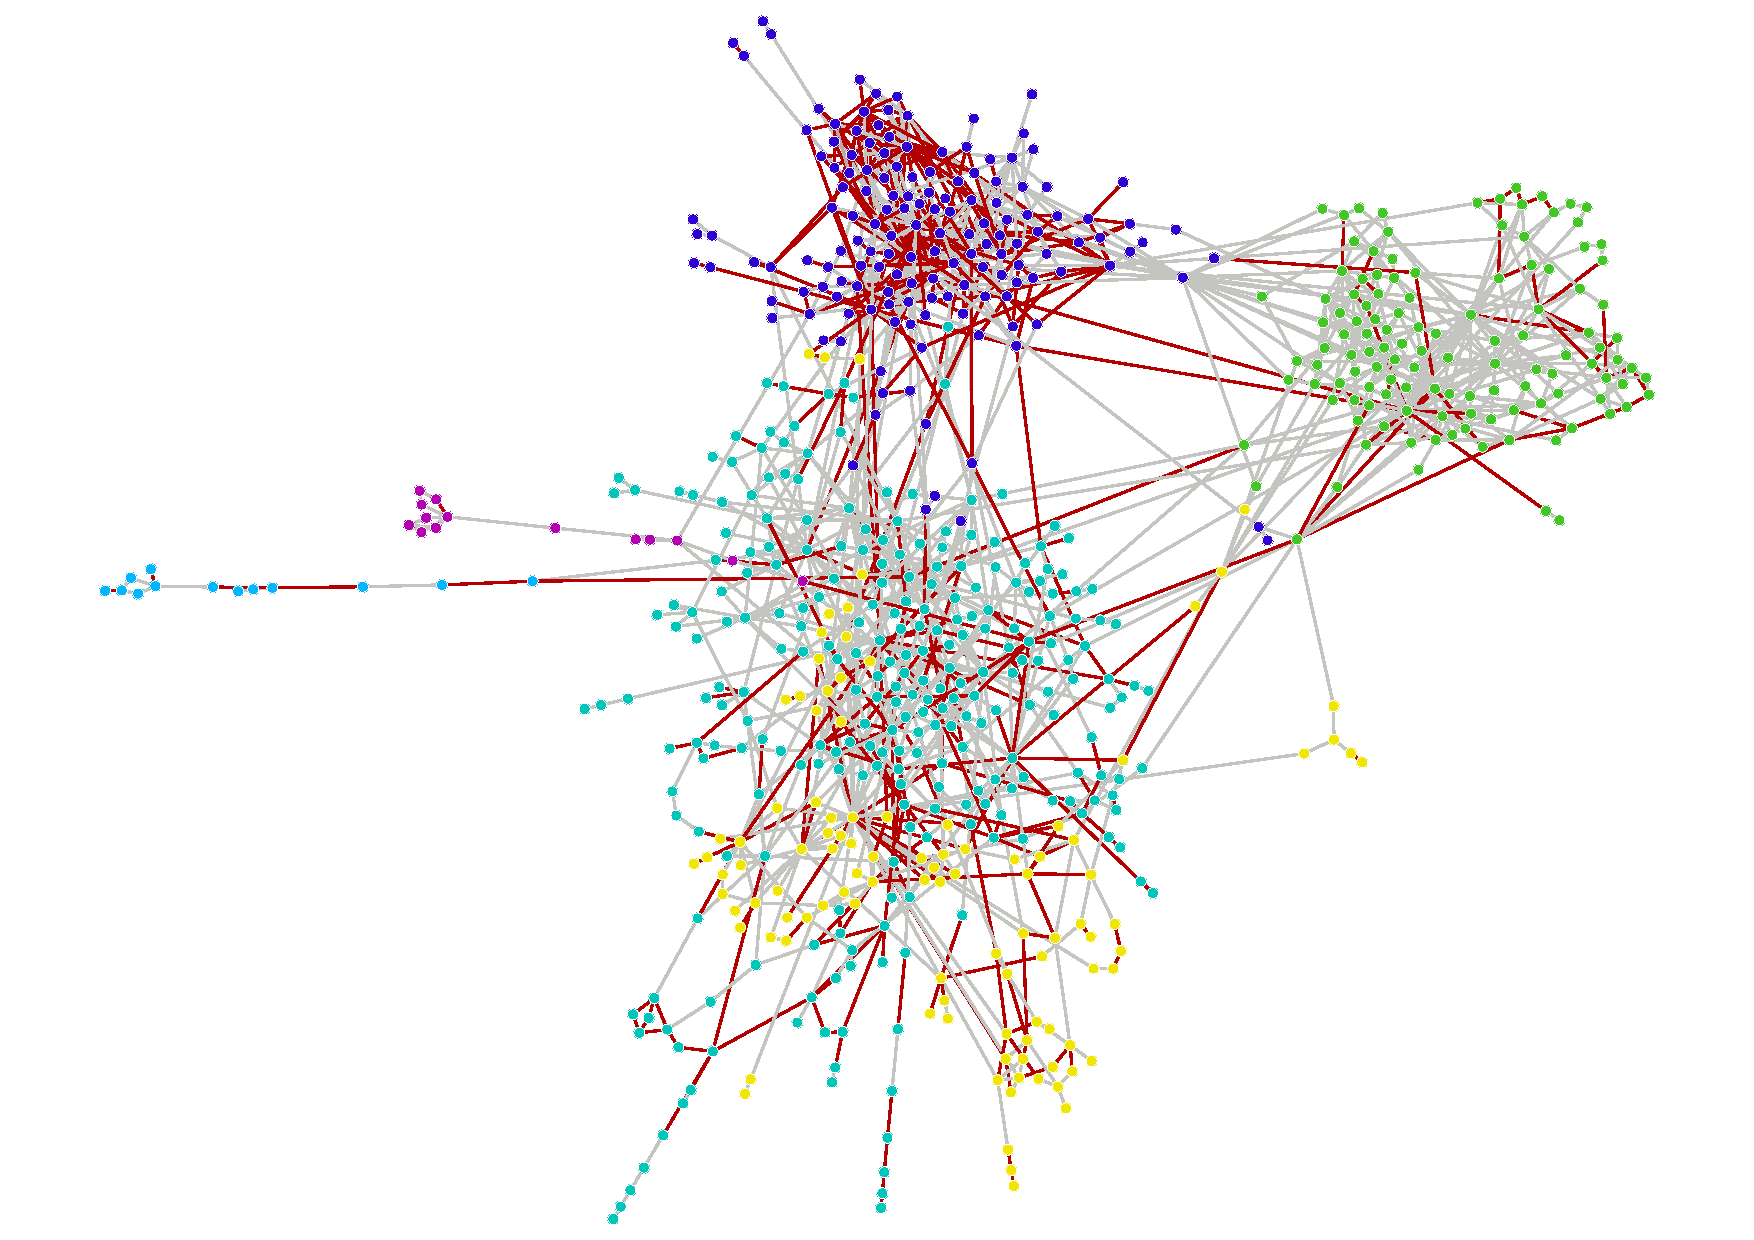
\includegraphics[width=\textwidth]{images/ted_networks/hu_2014_edge_clustered_sb.pdf}
  \caption[2014 Hungarian Procurement Market with Edge Communities]{The 2014 Hungarian procurement market. We plot the largest connected component of the network, filtering out nodes involved in less than three contracts for the sake of visualization. Nodes are buyers and suppliers of contracts, connected by an edge if they contract with one another. Edges are colored red if the single bidding rate on the edge exceeds the average rate of single-bidding that year. The node colors denote membership in the same edge community. For the sake of visualization we assign each node to the edge community most common among its adjacent edges. Single bidding is significantly over-represented among the edges in the top left cluster, consisting of pharmaceutical and medical contracts.}
  \label{fig:hu2014_edgecluster}
\end{figure*}

Motivated by this observation of cluster-level heterogeneity of single bidding, we calculate, for each country-year procurement market, a measure of the inter-cluster variance of single bidding. We first calculate a size-weighted coefficient of variation of single bidding rates across edge clusters in each network. Seeking to find an appropriate benchmark, we randomize single bidding across the network and recalculate the same coefficient of variation measure. As before, we do not randomize single bidding across all contracts blindly, rather we shuffle the single bidding label only within level-2 CPV codes, as we did with the benchmark for the concentration of single bidding in the network cores. Again we do this in order to allow for differences in the levels of competition between sectors.

Given a partition of the edges of the network, we naturally have a partition of the underlying contracts. We then calculate the coefficient of variation of single bidding rates across the clusters, defined as the ratio of the standard deviation ($\sigma_{SB}$) of single bidding to the mean of single bidding ($\mu_{SB}$) across clusters. Because the clusters vary significantly in size, we weight the contribution of each cluster to the standard deviation and mean of single bidding as follows:


$$\sigma^{W}_{SB} = \sqrt{ \frac{ \sum_{c\in C} |c| (sb_{c} - \mu^{W}_{SB})^2 }{ \frac{(|C|-1)}{|C|} \sum_{c\in C} |c| } },$$
and
$$\mu^{W}_{SB} =  \frac{\sum_{c \in C} |c| sb_{c}}{\sum_{c \ in C} |c|},$$

\noindent where $C$ is the set of contract clusters, $c$ is a specific cluster, and $sb_{c}$ is the rate of single bidding in the cluster $c$. The weighted coefficient of variation, which in our context we refer to as the clustering of single bidding, is simply the ratio $\sigma^{W}_{SB}/\mu^{W}_{SB}$.

As suggested, we wish to compare the observed clustering of single bidding against a plausible null model of within-sector randomized single bidding. For each market we randomize the single bidding label within the CPV-2 codes 1000 times and recalculate the same weighted coefficient of variation. We scale the observed clustering of single bidding against the average of these 1000 randomizations to arrive at a comparable measure of the extent which corruption is clustered. We again average over all years for each country, reporting the resulting values in Table~\ref{table:clustering_sb}. 

We plot the relationship between clustering of single bidding with both overall single bidding rates, and the relative size of the core of each country in Figure~\ref{fig:sbclustercompare}. We find only a weak relationship between the overall rate of single bidding and its tendency to cluster. We also observe a few interesting outliers: Romania, Latvia, Lithuania, and Poland have over five times the heterogeneity of single bidding across network clusters than expected under a conservative null model. Italy, with its relatively high rate of single bidding has one of lowest rates of clustering of single bidding. Among countries with lower single bidding rates, the UK, Germany, and France have relatively high rates of clustering, while Belgium and Sweden have relatively low rates. We find a stronger correlation between clustering of risk and centralization of procurement in the core of the network, driven mostly by the four outliers mentioned above.

\begin{table}
\begin{tabular}{lr}
\toprule
Country &  Normalized Clustering of Single Bidding\\
\midrule
BE      &                 2.03 \\
SE      &                 2.05 \\
IT      &                 2.09 \\
SI      &                 2.23 \\
PT      &                 2.30 \\
IE      &                 2.38 \\
FI      &                 2.42 \\
NL      &                 2.47 \\
AT      &                 2.56 \\
ES      &                 2.59 \\
DK      &                 2.60 \\
EE      &                 2.67 \\
CY      &                 3.04 \\
BG      &                 3.06 \\
FR      &                 3.34 \\
SK      &                 3.35 \\
DE      &                 3.45 \\
HU      &                 3.49 \\
CZ      &                 3.81 \\
UK      &                 4.08 \\
PL      &                 5.28 \\
LT      &                 5.47 \\
LV      &                 6.49 \\
RO      &                 7.22 \\
\bottomrule
\end{tabular}
\caption[Clustering of Single Bidding by Country]{Average clustering of single bidding within edge-communities of EU countries, normalized by a randomized sector-preserving null model of single bidding. Higher numbers indicate that single bidding rates are more heterogeneous across clusters.}
\label{table:clustering_sb}
\end{table}

\begin{figure*}
\centering
  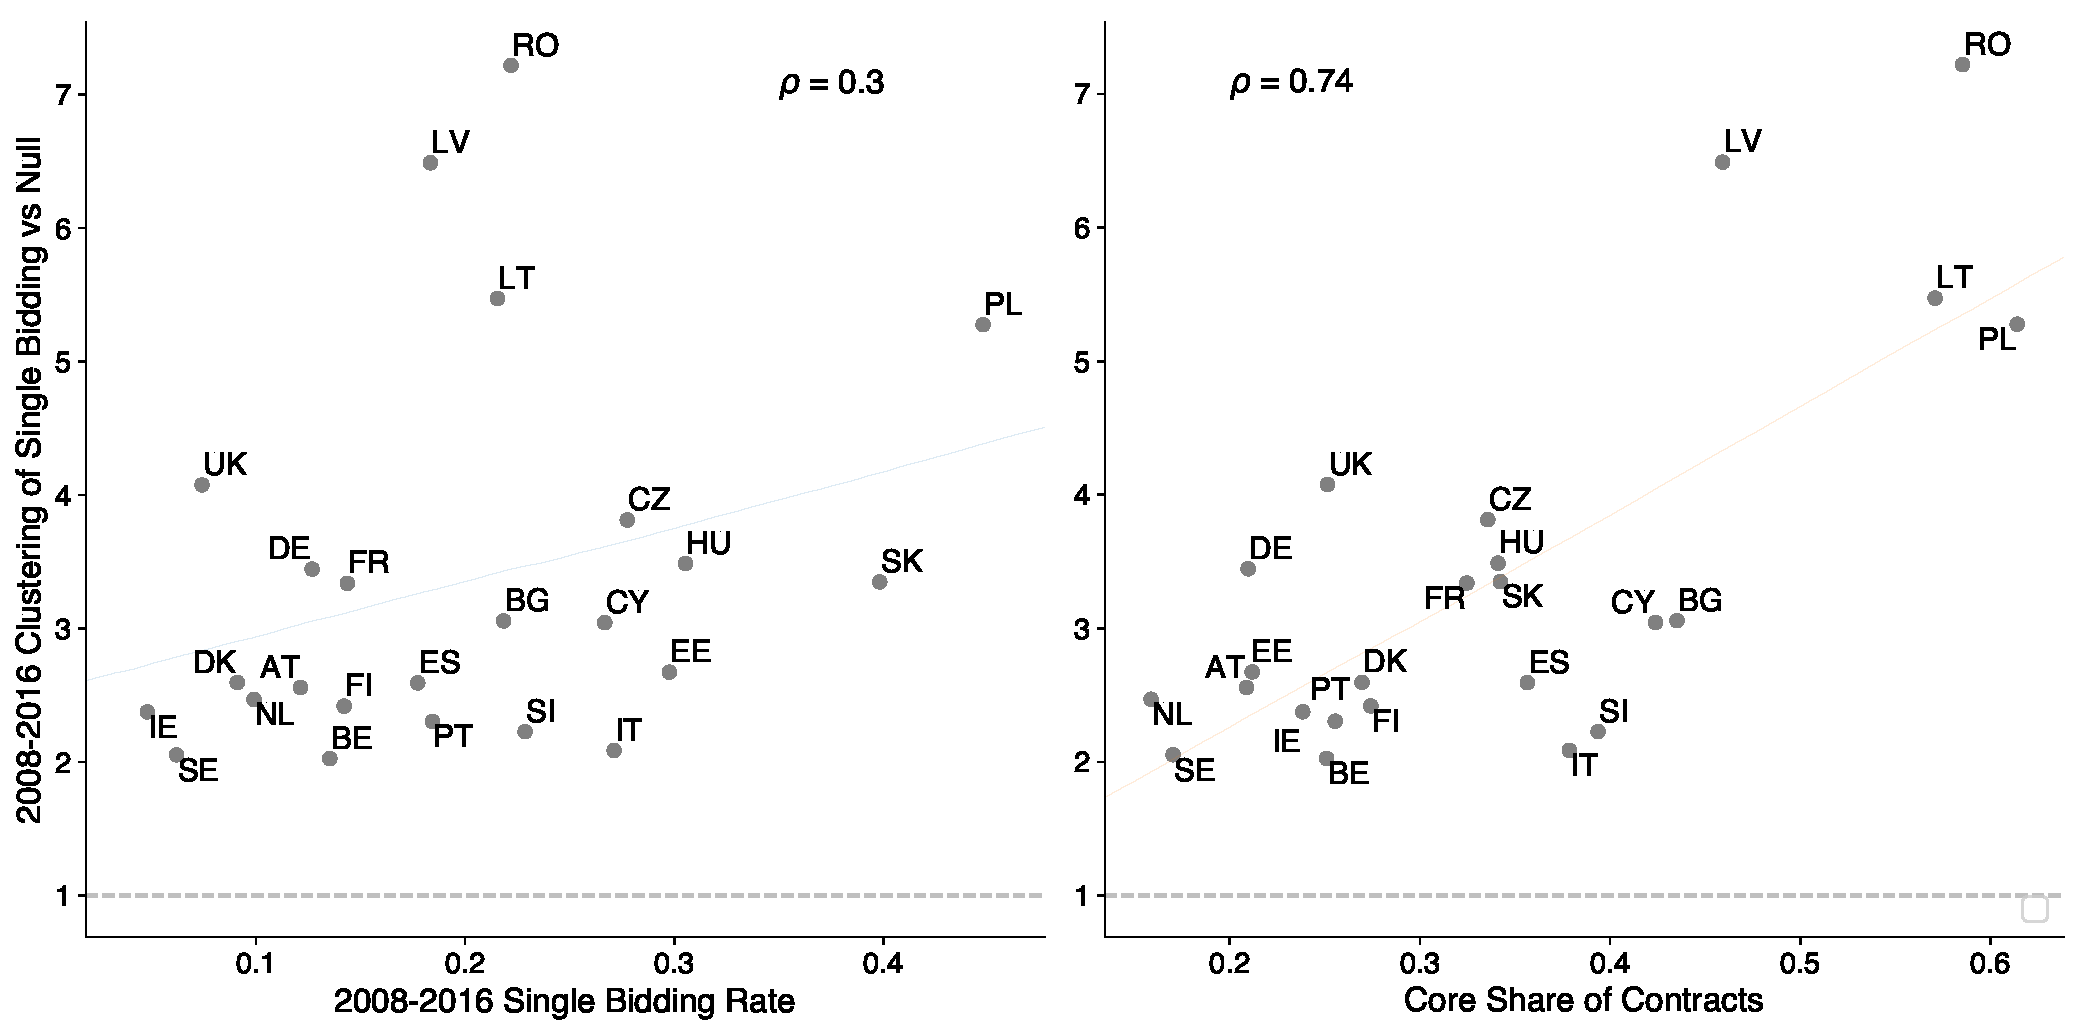
\includegraphics[width=\textwidth]{images/ted_networks/sbcluster_comparison.pdf}
  \caption[The scaled clustering of single bidding in a market, compared with its overall single-bidding rate and centralization.]{The scaled clustering of single bidding in a market, compared with its overall single-bidding rate and centralization. Averaged over 2008-2016, with Pearson correlations.}
  \label{fig:sbclustercompare}
\end{figure*}


We interpret these findings as indicating significant heterogeneity in the organization of corruption across the EU countries. In some countries corruption risk as measured by single bidding rates is highly concentrated in a few corners of the market, while in others it is much more evenly distributed. To underline the value of finding these heterogeneities, we claim that the right policy recommendations to counteract corruption depends crucially on understanding these patterns. As we saw in the visualization of the Hungarian market, one cluster clearly has higher rates of single bidding than do the others. Investigators, public or private, can immediately hone in on specific clusters in such a situation. In Italy, on the other hand, where the heterogeneity of single bidding across clusters is relatively low, a similar approach would have less value. There policymakers may be more interested in taking a decentralized approach to anti-corruption activities, for example by supporting whistleblowers and incentivizing the exposure of corruption by insiders.    


\subsection{Market Turnover and Change in Government}
In the final section of this chapter, we analyze the effect of changes in government on procurement markets. This is another potential source of heterogeneity in the organization of corruption in different contexts. Past work has found significant evidence of political cycles in procurement in countries such as Russia~\cite{mironov2016corruption}. Using the survival rate of procurement winners in the core, we can compare the turnover of frequent high single bid contract winners with other core firms across politically volatile and tranquil years. We find differences that again offer interesting theoretical insights and suggest different kinds of policy interventions.


\begin{table}[t]
\begin{tabular}{lr}
\toprule
Country &                           Year \\
\midrule
BG      &              2009, 2013, 2014 \\
CY      &                          2013 \\
CZ      &        2009, 2010, 2013, 2014 \\
DK      &                    2011, 2015 \\
ES      &                          2011 \\
FR      &                          2012 \\
GR      &              2009, 2012, 2015 \\
HU      &                          2010 \\
IE      &                          2011 \\
IT      &        2006, 2008, 2011, 2013 \\
LT      &                          2012 \\
NO      &                          2013 \\
PL      &                    2007, 2015 \\
PT      &                    2011, 2015 \\
RO      &              2008, 2012, 2015 \\
SE      &                    2006, 2014 \\
SI      &                          2012 \\
SK      &              2006, 2010, 2012 \\
UK      &                          2010 \\
\bottomrule
\end{tabular}
\caption[Changes of Government, EU countries]{Substantial changes of government in EU countries, 2006-2017. We code a change of government if the head of the government (i.e. chancellor, prime minister) changes, and if all parties involved in government change. Source: ParlGov database (Döring and Manow 2018)}
\label{table:changes_of_gov}
\end{table}

We define change in government using data from the ParlGov database on cabinets~\cite{doring2010parliament}, reported in Table~\ref{table:changes_of_gov}. We say that a country experienced a change in government in a specific year, if the head of the government (for example the prime minister or chancellor) and all parties participating in the government changed. This is a rather conservative definition of change in government. For example, if a junior coalition party leaves the government or if a prime minister is replaced by a technocratic government with support by the same parties, we do not consider this a change in government. One drawback to this approach is that some countries, for example Germany and Austria, did not have, by our definition, a change of government in the span of our dataset. Despite our restrictive definition, some countries with more volatile political cycles (Italy or Czechia for example) had multiple changes of government. In any case, political turbulence is itself an important indicator of political health of a country, with past work indicating that political stability is correlated with lower levels of corruption~\cite{lederman2005accountability}. On the other hand, extreme stability may indicate a lack of political competition and we observed in Chapter 3 that Hungarian settlements with weaker political competition had higher rates of corruption risk in their contracts. Though researchers have developed increasingly granular, social media-based measures of political volatility or ``turbulence''~\cite{margetts2015political}, we stick with our top down approach. 

Another limitation of our method of analysis is that we only consider central government changes. Many countries in Europe have significant federal structures with significant devolution of political responsibilities. We mitigate limitation this by focusing our efforts on contracts in the core of the network, which are more likely to involve central government attention, directly or indirectly.

For each year from 2008 to 2014, we collect the core winners of each market, as defined in the previous section. We calculate their survival (as either a core or periphery winner of public contracts in that country) two years later. We use a two year gap to give room for potential changes of government to happen in the intervening year. We split the core winners into two groups: those with above and below average single bidding rates (where the average is calculated only among core contracts). We present the Hungarian case in Figure~\ref{fig:hu_core_turnover}, observing a steep drop in the survival rate of core winners with high single bidding rates across the 2010 elections. This suggests a significant turnover of favored firms in the Hungarian case, with particularist contract steering as a potential mechanism.

\begin{figure*}
\centering
  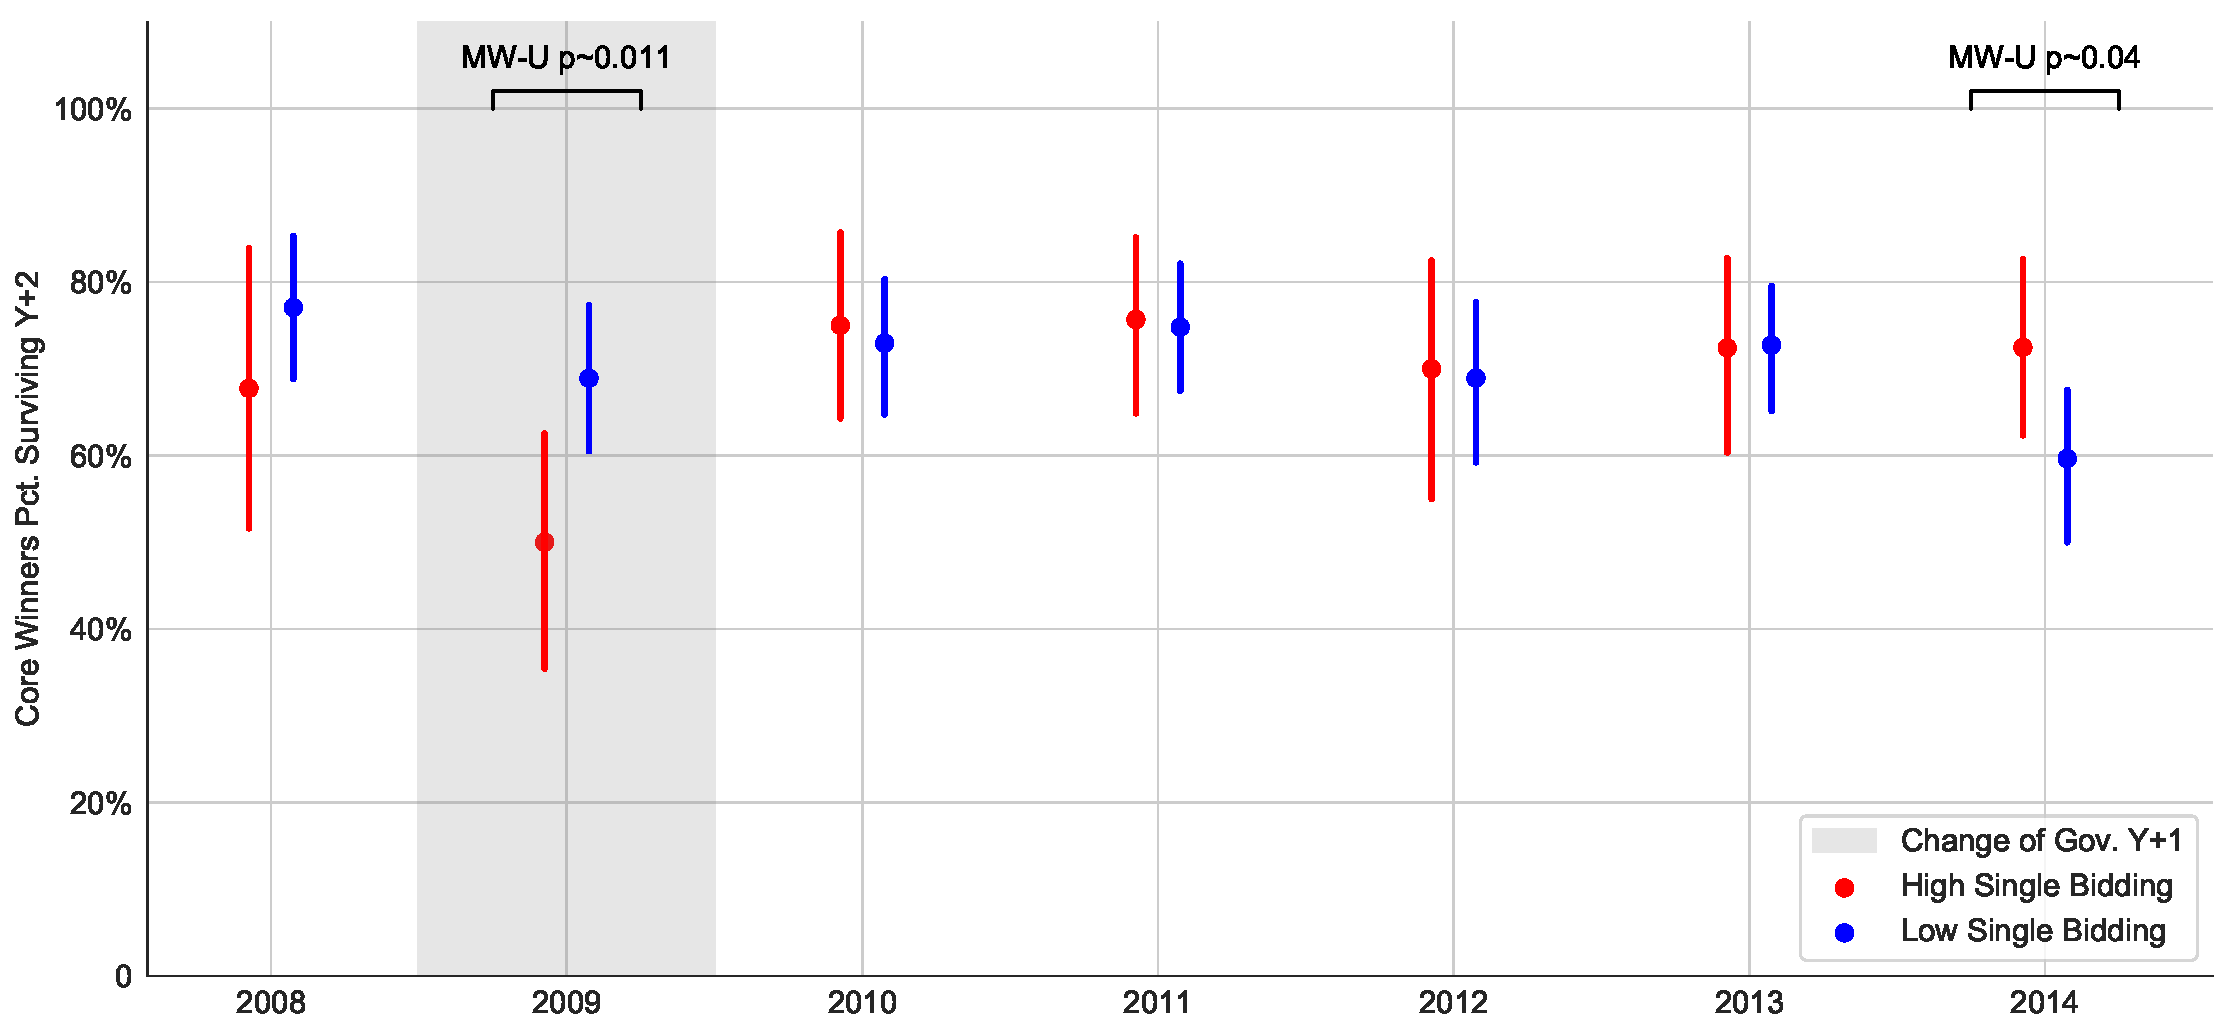
\includegraphics[width=\textwidth]{images/ted_networks/hu_cog_core.pdf}
  \caption[Hungarian procurement market turnover]{The two year survival rates of Hungarian core winners, split up by above and below average single bidding rates. When significant, a Mann-Whitney U test of the difference in means is reported. 2009, the year preceding a change in government in Hungary is highlight in grey.}
  \label{fig:hu_core_turnover}
\end{figure*}

How do the other EU countries compare? We now outline a method to compare the differences in survival rates of winners with high and low single bidding rates across years of change of government and other years. Explicitly, we compare the ratio of the survival rates of high to low risk winners across change in governments, $S_{CoG}^{H}/S_{CoG}^{L}$, and the same ratio in other years: $S_{\lnot CoG}^{H}/S_{\lnot CoG}^{L}$. The ratio of these ratios can be interpreted as a kind of ~\textit{survival premium} that high single bidder winners have across changes of government, relative to their low single bidder counterparts. We estimate the statistical significance of this premium using the bootstrap~\cite{efron1994introduction}. Specifically, we sample the survival outcomes of each of the four pools of winners (high and low single bidders and across or away from changes in government) with replacement and recalculate the ratio a thousand times for each country, generating a confidence interval for our estimate of the survival premium of high single bidder winners across changes in government. We interpret countries with the 95\% confidence interval of the ratio entirely below 1 (as we shall soon see is the case for Hungary) as those countries in which corrupt arrangement are vulnerable to political turnover. Countries in which the interval is entirely above one have corruption organized in a way that is robust to political turnover. Finally, when the 95\% confidence overlaps with 1, we say that corruption in the country is neither vulnerable nor robust to political turnover.

We plot the estimates and intervals for each country in Figure~\ref{fig:core_sb_cog_surv}, sorted in increasing order. Echoing the previous sections we find some surprising differences between the countries in our sample. High corruption risk winners in Hungary, Greece, Spain, Italy, Portugal, Denmark and France (though the effect size of France is not large) have significantly more turnover compared to their low risk counterparts when there is a change in government than otherwise. The opposite is true for Romania, Poland, and Sweden. For the remainder of the countries, the effect is not significant.

\begin{figure*}
\centering
  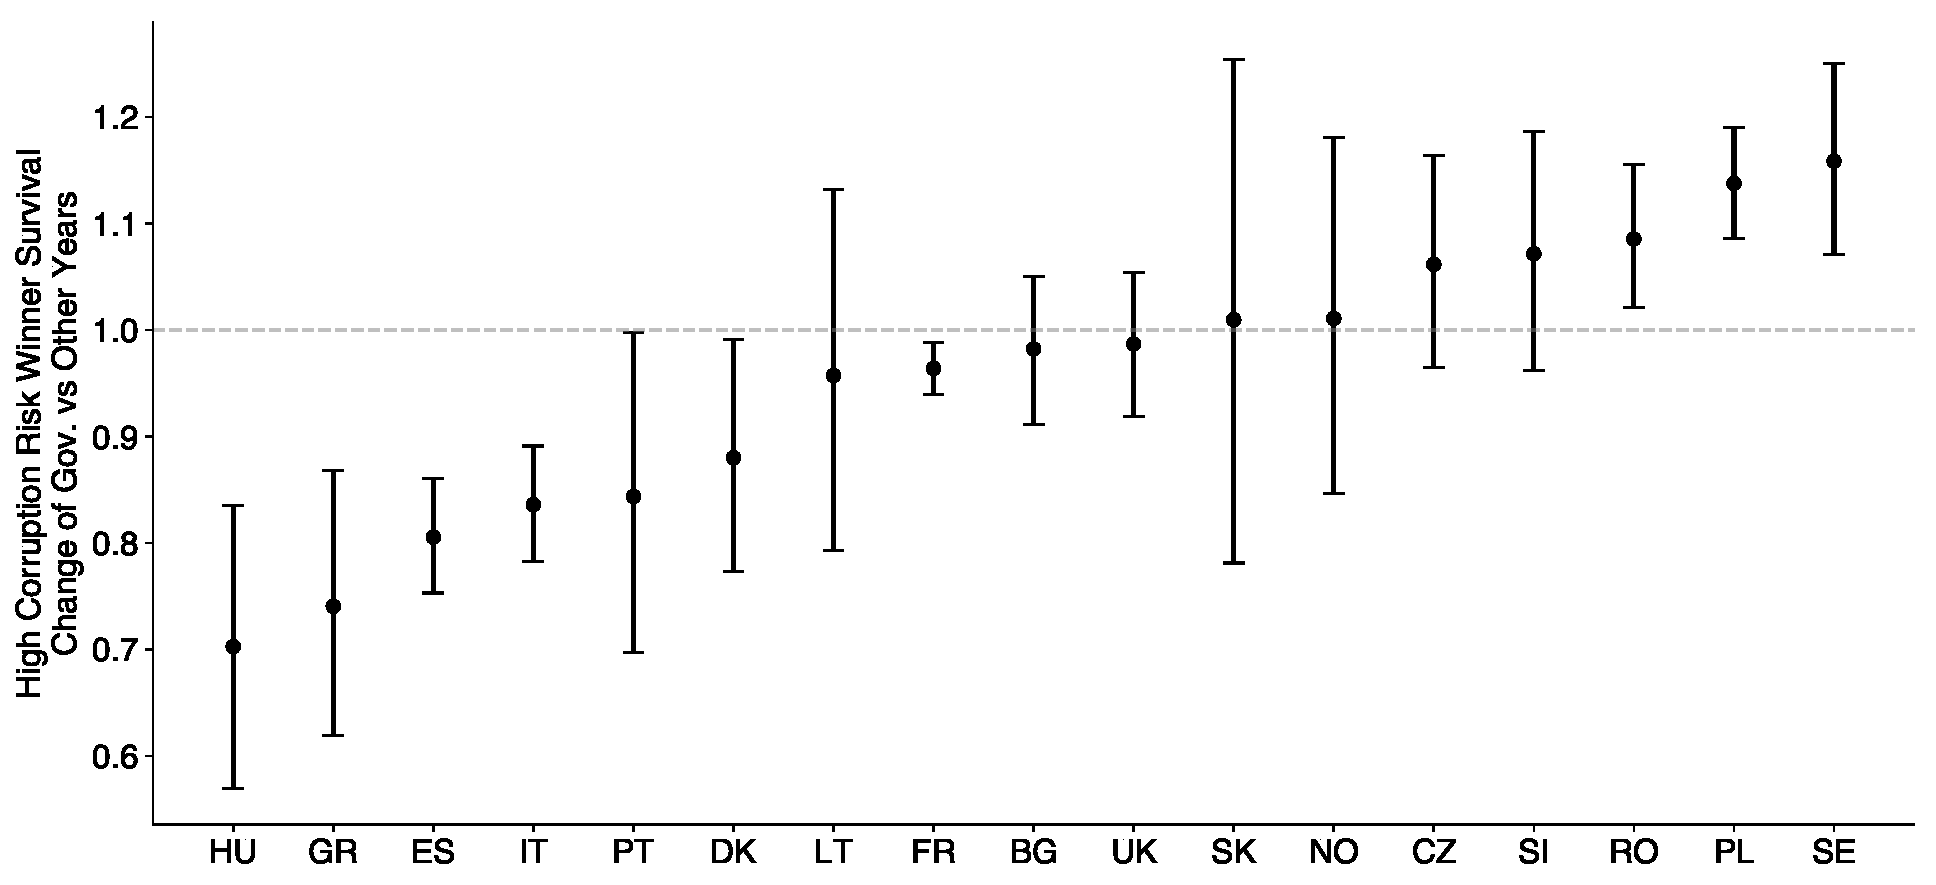
\includegraphics[width=\textwidth]{images/ted_networks/core_sb_cog_survival.pdf}
  \caption[Political turnover and corrupt winner turnover]{The two-year survival premium of core winners with high rates of single bidding across change of government vs other years. Low values indicate that winners of relatively many single bid contracts are less likely to survive across a change in government than across other two year periods. High values indicate that such winners are rather robust to change in government.}
  \label{fig:core_sb_cog_surv}
\end{figure*}

That corrupt winners are robust to political volatility in Romania and Poland presents a puzzle. In the former socialist countries of Central Eastern Europe, corruption and state capture are often described as the results of an ideological competition between elites who seek to extract rents from the state, which Innes refers to as the ``great electoral lottery''~\cite{innes2002party}. With such a framing one would expect more turnover of high corruption risk winners across changes in government, as the elite rewire the rent extracting connections between institutions and firms. An alternative framing could be that in Romania and Poland, corruption works along non-ideological lines, with corrupt actors simply engaging with whoever is in charge, and embedding themselves into the system in a way that ensures survival regardless of political outcome. This idea has some theoretical support in Romania, where MPs frequently and opportunistically switch parties~\cite{fieruascu2018exploring}. Poland, however, is usually presented as a polarized society in which political competition is highly ideological~\cite{grzymalala2003great}. Polish voters are especially likely to mobilize because of corruption perceptions~\cite{slomczynski2012perceptions}. This finding certainly merits further study.

On the other hand it is quite interesting that corruption risk implies increased volatility consistently among Hungary and the Mediterranean countries, in contrast with both the rest of Eastern Europe and Northern Europe. We briefly consider implications for policymakers given these heterogeneities. In countries in which corrupt firms are vulnerable to political turnover, it is likely that staggering local and regional elections may have a virtuous effect on the overall level of corruption, as suggested by previous work comparing the Czech Republic (where elections are entirely asynchronous) and Hungary (where elections are highly synchronized)~\cite{fazekas2017networks}. By increasing volatility across levels of government, it makes it harder to organize corruption, for example because it is more likely that an important election is imminent at any given time and that voters can punish misbehaving political parties more quickly and consistently. In Romania and Poland, where we found the opposite tendency, it is rather likely that personal ties and brokers between firms and political parties are enabling the survival of high corruption risk winners across elections.



\section{Discussion}


In this chapter we studied the relationship between corruption risk and procurement market structure in EU countries. By observing centralization, clustering, and turnover of the market using network methods, we describe the organization of corruption in novel ways. Our approach highlights the multifaceted nature of corruption. With the exception of a strong correlation between centralization in a market and its rate of single bidding, we do not generally find clear relationships between the overall prevalence of corruption risk in a country and the structure of its procurement market.  For example, in some countries corruption risk is more prominent in the core of the procurement market, while in others it is rather over-represented in the periphery. In all countries we found that corruption risk is distributed across sub-markets in a non-random way, but the extent to which this is true varies greatly. Finally, we found that winners of corruption contracts react very differently to changes in government in different countries around the EU. 

Not only are these distinctions theoretically important, but they suggest practical implications for anti-corruption actors from activist to prosecutor. The network approach builds up from micro-level interactions to describe emergent structure - in this case highlighting significant national-level differences in procurement markets. They also suggest several avenues for further research. One could for instance focus on specific countries, just as this chapter has tended to use Hungary as an example. The hypotheses of country-level experts on the nature of corruption in specific societies could be tested using our framework. It could also be extended to compare non-EU countries, depending on the comparability of the data. Finally, we note that in future work a greater emphasis on the temporal evolution of these markets and their actors is merited. For instance, an analysis of market structure can give a much more real-time measure of change in corruption risk than can survey-based perception measures, which are often a lagging indicator of such effects. Such a perspective is crucial to discovering the causal mechanisms and directions behind the relationships we have discovered in this chapter, for if procurement market decentralization causes a decrease in corruption.

